% Options for packages loaded elsewhere
\PassOptionsToPackage{unicode}{hyperref}
\PassOptionsToPackage{hyphens}{url}
\PassOptionsToPackage{dvipsnames,svgnames,x11names}{xcolor}
%
\documentclass[
  10pt,
]{scrbook}
\usepackage{amsmath,amssymb}
\usepackage{lmodern}
\usepackage{iftex}
\ifPDFTeX
  \usepackage[T1]{fontenc}
  \usepackage[utf8]{inputenc}
  \usepackage{textcomp} % provide euro and other symbols
\else % if luatex or xetex
  \usepackage{unicode-math}
  \defaultfontfeatures{Scale=MatchLowercase}
  \defaultfontfeatures[\rmfamily]{Ligatures=TeX,Scale=1}
\fi
% Use upquote if available, for straight quotes in verbatim environments
\IfFileExists{upquote.sty}{\usepackage{upquote}}{}
\IfFileExists{microtype.sty}{% use microtype if available
  \usepackage[]{microtype}
  \UseMicrotypeSet[protrusion]{basicmath} % disable protrusion for tt fonts
}{}
\makeatletter
\@ifundefined{KOMAClassName}{% if non-KOMA class
  \IfFileExists{parskip.sty}{%
    \usepackage{parskip}
  }{% else
    \setlength{\parindent}{0pt}
    \setlength{\parskip}{6pt plus 2pt minus 1pt}}
}{% if KOMA class
  \KOMAoptions{parskip=half}}
\makeatother
\usepackage{xcolor}
\IfFileExists{xurl.sty}{\usepackage{xurl}}{} % add URL line breaks if available
\IfFileExists{bookmark.sty}{\usepackage{bookmark}}{\usepackage{hyperref}}
\hypersetup{
  pdftitle={Modeling Mindsets for Data Scientists},
  pdfauthor={Christoph Molnar},
  colorlinks=true,
  linkcolor={Maroon},
  filecolor={Maroon},
  citecolor={Blue},
  urlcolor={Blue},
  pdfcreator={LaTeX via pandoc}}
\urlstyle{same} % disable monospaced font for URLs
\usepackage{longtable,booktabs,array}
\usepackage{calc} % for calculating minipage widths
% Correct order of tables after \paragraph or \subparagraph
\usepackage{etoolbox}
\makeatletter
\patchcmd\longtable{\par}{\if@noskipsec\mbox{}\fi\par}{}{}
\makeatother
% Allow footnotes in longtable head/foot
\IfFileExists{footnotehyper.sty}{\usepackage{footnotehyper}}{\usepackage{footnote}}
\makesavenoteenv{longtable}
\usepackage{graphicx}
\makeatletter
\def\maxwidth{\ifdim\Gin@nat@width>\linewidth\linewidth\else\Gin@nat@width\fi}
\def\maxheight{\ifdim\Gin@nat@height>\textheight\textheight\else\Gin@nat@height\fi}
\makeatother
% Scale images if necessary, so that they will not overflow the page
% margins by default, and it is still possible to overwrite the defaults
% using explicit options in \includegraphics[width, height, ...]{}
\setkeys{Gin}{width=\maxwidth,height=\maxheight,keepaspectratio}
% Set default figure placement to htbp
\makeatletter
\def\fps@figure{htbp}
\makeatother
\setlength{\emergencystretch}{3em} % prevent overfull lines
\providecommand{\tightlist}{%
  \setlength{\itemsep}{0pt}\setlength{\parskip}{0pt}}
\setcounter{secnumdepth}{5}
% Geometry
\usepackage[paperwidth=18.9cm, paperheight=24.61cm, inner=30mm, outer=17mm, top=30mm, bottom=24mm]{geometry}


% Decide for a font
%\usepackage{Alegreya}
%\usepackage[scale=.7]{sourcecodepro}


% Make stuff less floaty
\renewcommand{\textfraction}{0.05}
\renewcommand{\topfraction}{0.8}
\renewcommand{\bottomfraction}{0.8}
\renewcommand{\floatpagefraction}{0.75}

% For proofreading: Big margin on the right and 2x linespace
%\linespread{2}
%\geometry{
%  a4paper,
%    total={189mm,246mm},
%  left=20mm,
%  top=20mm,
%  right=70mm,
%  asymmetric
%}

% Header and footer configuration
\usepackage[automark,headsepline]{scrlayer-scrpage}
% Use scrpage2 instead of scrlayer-scrpage if you want to nicer chapter boxes, see main/main.tex. --- WILL NOT WORK WITH TEXLIVE 2019! ----
%\usepackage[automark,headsepline]{scrpage2}
\pagestyle{scrheadings}
\ihead[\headmark]{\headmark}\ohead{\pagemark}
% alternating chapter / section titles at the top of the page
\automark[section]{chapter}
% Make heading of each page italics and small capitals.
\renewcommand*{\headfont}{\itshape\scshape}
% Name of the chapter (\chapapp), number of the chapter (\thechapter) and no period (\autodot)
\renewcommand*{\chaptermarkformat}{\chapapp~\thechapter\autodot\enskip}
% Removes page numbers from bottom
\ofoot{}


% Turns href urls into foodnotes
\let\oldhref\href
\renewcommand{\href}[2]{#2\footnote{\url{#1}}}

% Create index
\usepackage{makeidx}
\makeindex

% Pages for publishing, like empty pages
\frontmatter
\ifLuaTeX
  \usepackage{selnolig}  % disable illegal ligatures
\fi

\title{Modeling Mindsets for Data Scientists}
\author{Christoph Molnar}
\date{2022-04-26}

\begin{document}
\maketitle

%\cleardoublepage\newpage\thispagestyle{empty}\null
%\cleardoublepage\newpage\thispagestyle{empty}\null
%\cleardoublepage\newpage
\thispagestyle{empty}
%\begin{center}
%\includegraphics{images/dedication.pdf}
%\end{center}

%\setlength{\abovedisplayskip}{-5pt}
%\setlength{\abovedisplayshortskip}{-5pt}


% =========================================================================
% Title page with cover
% =========================================================================

\iffalse
\thispagestyle{empty}

\vspace{3cm}
  \begin{center}
    {
	\bfseries \sffamily \Huge Modeling Mindsets for Data Scientists \par
	\bfseries \LARGE The Many Cultures of Learning From Data \par
~\\
	~\\
	\bfseries \small Published by Christoph Molnar, Munich\par
      }
  \end{center}


\newpage
\fi
% =========================================================================
% Page with publishing details
% =========================================================================



\thispagestyle{empty}
\begin{center}
  {
  \bfseries \sffamily \LARGE Modeling Mindsets for Data Scientists \par
  \bfseries \small The Many Cultures of Learning From Data  \par
}

\copyright~2022 \textit{Christoph Molnar}, Germany, Munich\\
\url{christophmolnar.com}

For more information about permission to reproduce selections from this book, write to \url{christoph.molnar.ai@gmail.com}.

	\the\year, Second Edition

% Impression line, indicating number and year of current printing
% International Standard Book Number (ISBN)
% International Standard Serial Number (ISSN), if applicable
\ifxetex
	\textsc{ISBN 9798411463330 (paperback)} 
\fi


\includegraphics{images/by-nc-sa.png}

This book is licensed under the Creative Commons Attribution-NonCommercial-ShareAlike 4.0 International License.
% For translations, indication of original-language title, publisher, and copyright, acknowledgments, permissions, and other credits, including acknowledgment of grants, if applicable and space permitting
  
  Christoph Molnar,
  c/o Mucbook Clubhouse,
  Westendstraße 78,
  80339 München, Germany

\end{center}

% =========================================================================
% Dedication / Empty page before outline
% =========================================================================
\newpage
\thispagestyle{empty}
\mbox{}
\newpage








{
\hypersetup{linkcolor=}
\setcounter{tocdepth}{1}
\tableofcontents
}
\hypertarget{summary}{%
\chapter*{Summary}\label{summary}}


Modeling Mindsets is an introduction to the many modeling mindsets that you can use to understand and predict your data.

Statistics, machine learning, causal inference, Bayesianism, \ldots{}
The best modelers, researchers and data scientists don't stubbornly stick to only one mindset.
The best choose the right mindset for the right data task.

The book covers various mindsets, and each one gives you another superpower:
Statistical modeling, the foundation for many mindsets built on probability.
Frequentist inference as a decision-oriented tool.
Bayesian inference, a holistic probabilistic modeling approach.
Causal inference, a mindset that builds causality into your models.
Supervised machine learning, a mindset focused on prediction.
And many more.

Modeling Mindsets gives an introduction to all these different mindsets.
The book is packed with intuition, memorable illustrations, and strengths and limitations for each modeling mindset.
Expand your horizons in modeling and become a jack-of-all-trades in learning from data.

\hypertarget{what-this-book-is-about}{%
\chapter{What This Book is About}\label{what-this-book-is-about}}

The book introduces many modeling mindsets: each presents a different perspective on how to see the world through data.
It's an introduction to each mindset: its \emph{assumptions, central ideas, its relationship to other mindsets, and its strengths and limitations}.
The book is not about history and (formal) philosophy.
It's also not a full introduction to the mindsets.
After reading this book, you will not be a Bayesian, or any other type of modeler.
Modeling Mindsets can open the doors to new ways of thinking about modeling for you.
But there are other resources to explore what's behind each door -- an online course on machine learning, blog posts about about causal inference, a book about Bayesian inference, \ldots{}

\hypertarget{who-this-book-is-for}{%
\section{Who This Book is For}\label{who-this-book-is-for}}

The book is for data scientists, statisticians, machine learner, quantitative researchers, \ldots{}
In short, for anyone who already has experience with modeling data.
This means you probably already know one of the mindsets.
Perhaps, like me, you studied frequentist statistics.
Or you may be a researcher who has learned to use Bayesian inference to analyze your data.
Or maybe you are a self-taught machine learner.
A little bit of math should not scare you off.

\mainmatter

\hypertarget{models}{%
\chapter{Models}\label{models}}

Imagine you sit in front of some data and some questions that you are supposed to answer with help of the data.
You are asked to predict which patients might get side effects from this a drug.
How do bee colonies react to changing climate conditions?
Which supermarket products are always out-of-stock?
Data alone can tell you what happened: patients 124 and 22 got acne; 2/3 of bee colonies had troubles during drought in year 2018; on this one Tuesday the flour was sold out;
But usually you want to find general rules and relationships in the data.
Is flour low on stock at the beginning of the week in general?
Even better, these rules and relationships would extend not only to your sample, but to all patients / bee colonies / supermarkets.
To get from data to generalizable relationships, we have to simplify the real world and make assumptions.
The thing that helps us answer all the questions about our data is called a model.

A model is a simplified representation of something.
In the context of learning from data about the world, a model represents simplified aspects of the world.
The motivation to build or learn a model is that it allows us to answer questions and make predictions.

In this book we study specific types of models:
The models have to be computational or mathematical models.
This excludes, for example, physical models, like the tiny houses that architects build.
The second restriction: The models are learned from data.
This excludes ``designed'' models such as pure simulations like cellular automata.

There are three ingredients to a mathematical model:
A mathematical model contains \emph{mathematical structures} that represent \emph{variables} and put them in \emph{relation} (Figure \ref{fig:model}). \footnote{Weisberg, Michael. Simulation and similarity: Using models to understand the world. Oxford University Press, 2012.}
When a mathematical model is learned from data, it also contains \emph{parameters} that make the mathematical formula adaptable to data.
Furthermore, if you want to interpret models instead of the world, you have to make assumptions about the relationship between the model and aspects of the world.
But more on that in the \protect\hyperlink{mindsets}{mindsets chapter}.

\begin{figure}

{\centering 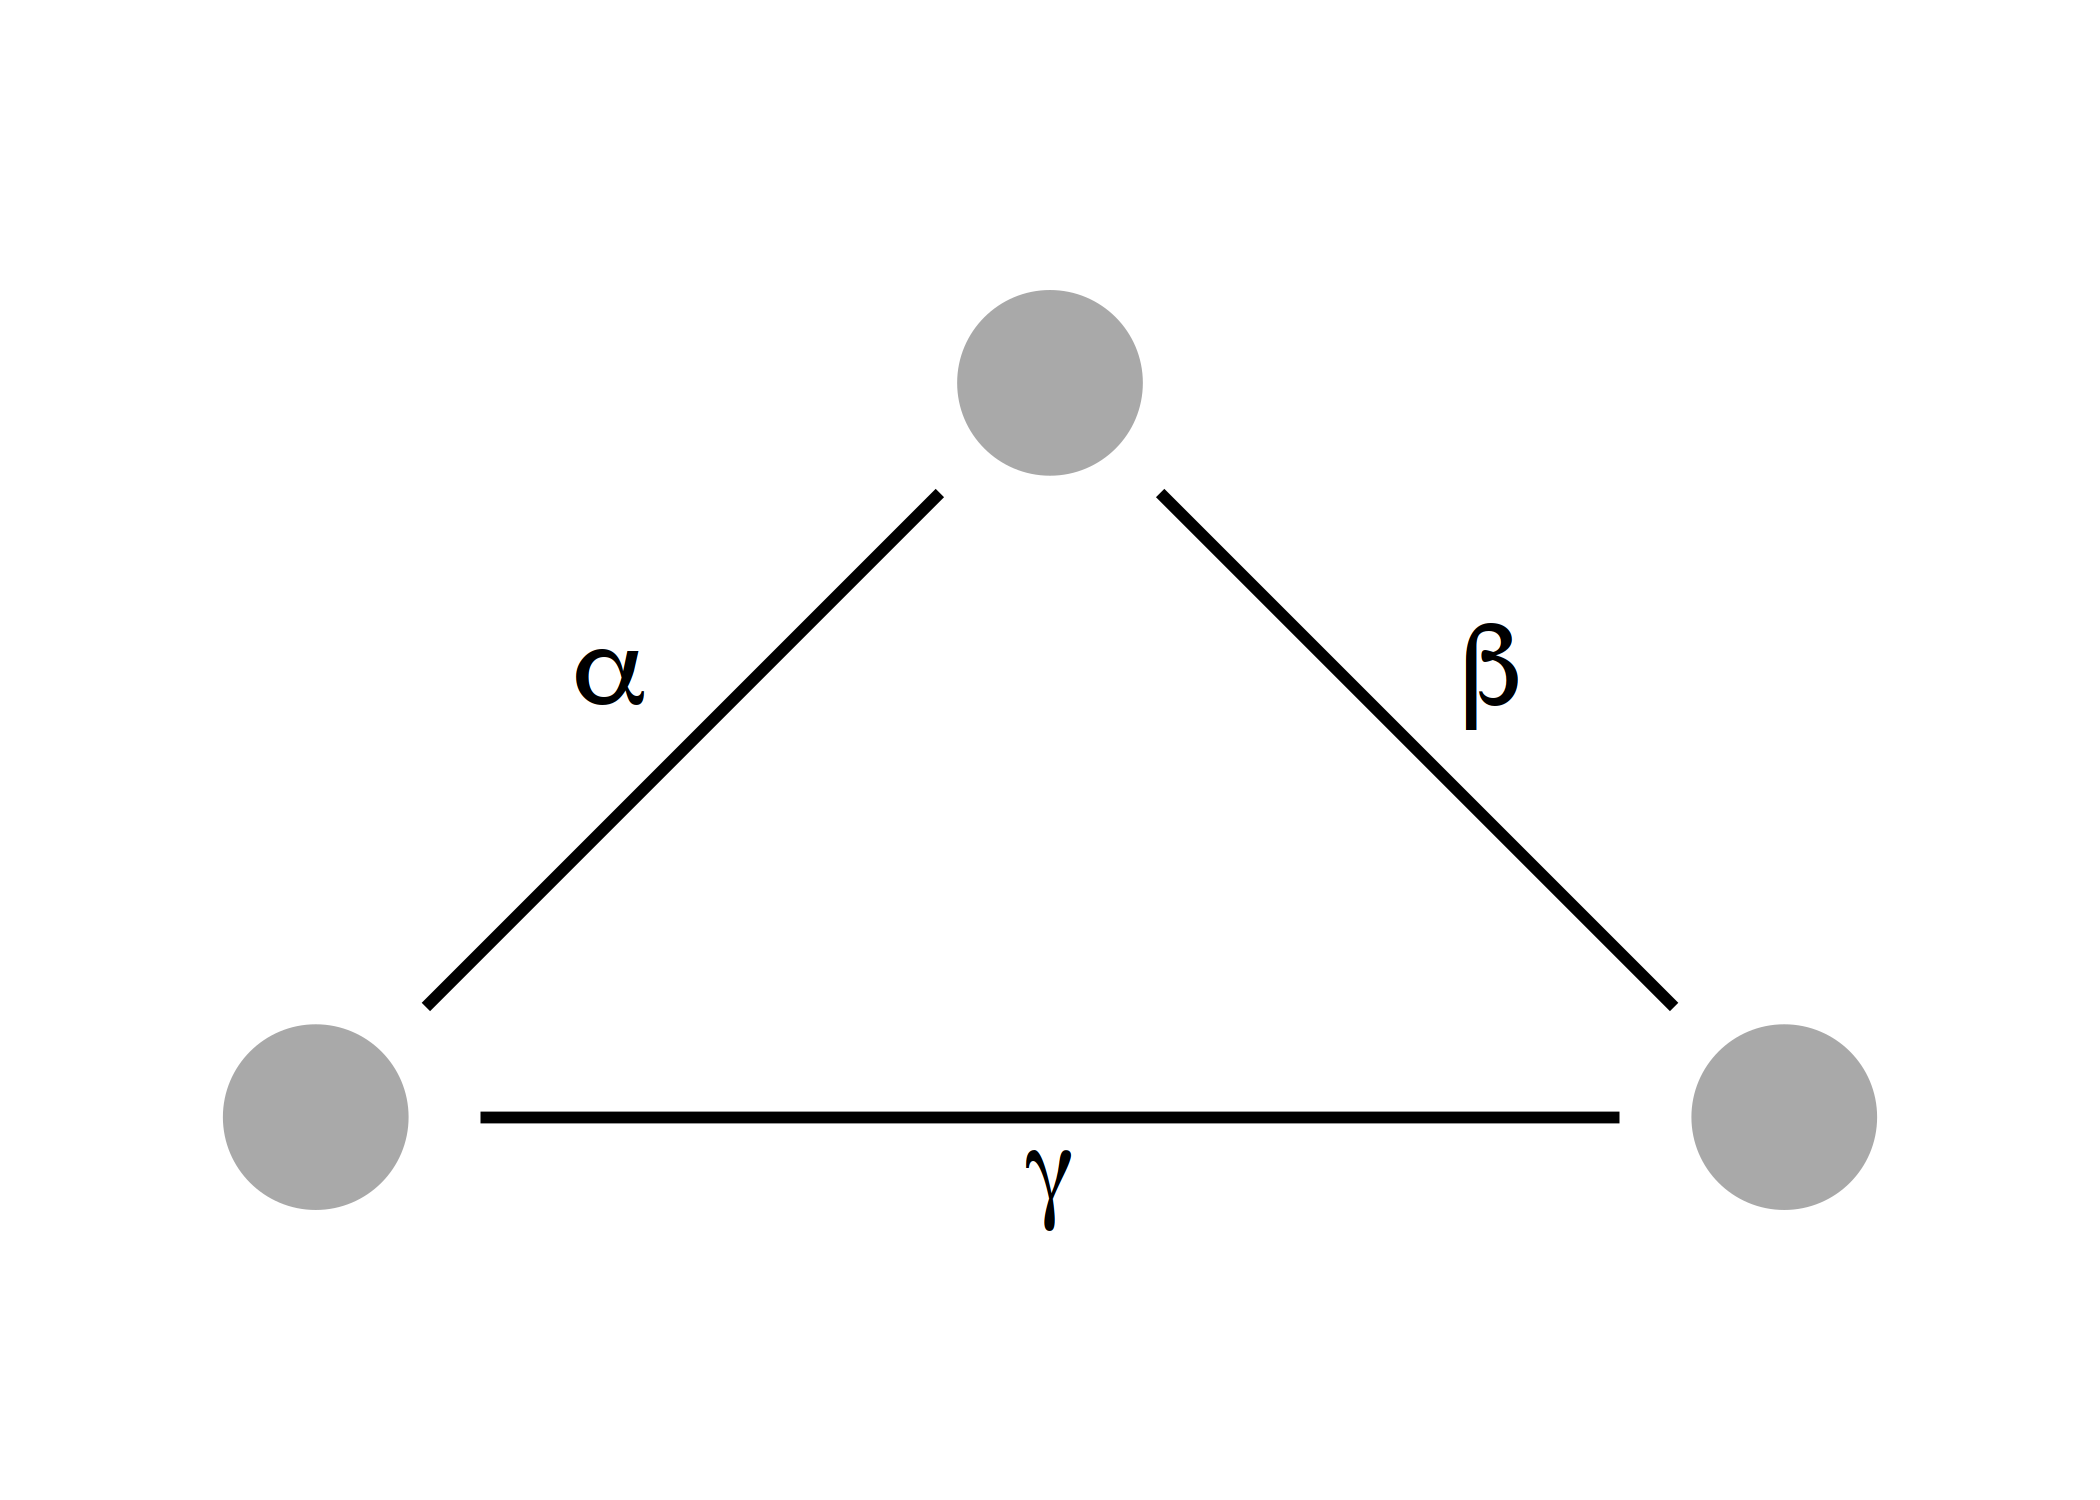
\includegraphics[width=0.8\textwidth]{figures/model-1} 

}

\caption{A mathematical model sets variables (dots) into relation (lines) using parameters.}\label{fig:model}
\end{figure}

The aspects of the world are represented within the model as \emph{variables}.
Images, for example, are represented as tensors of pixels.
The blood pressure of a patient is represented with a number for the model to use.
Variables can also represent a latent, hidden or abstract aspect.
Like happiness or introversion.
There are different names for these variables:
Random variables, covariates, predictors, latent variables, features, target, outcome, \ldots{}
These names sometimes reveal the role a variable takes on in our model, and are dependent on the modeling mindset we are in.
For example, in machine learning the word feature and target are used.
In statistics for similar variable roles, we would use independent and dependent variable, or covariates and outcome, \ldots{}

Within the model, the components are mathematically or computationally set in \emph{relation} to each other.
For example, causal models represent relations between variables as directed acyclic graph that can be translated into conditional (in-)dependencies.
The joint distribution of variables describes the occurrence of certain variable values in a probabilist sense.
A predictive model represents the output variable as a function of the input variables, in the case of a linear regression model as the sum of the input variables.

The expressive power of such relationships really depends on the class of the model.
A relationship can be a simple linear equation like \(Y = 5 \cdot X\) involving two or more variables.
For example we might model the probability of a stroke as a function of blood pressure and age.
A relationship can also be a long chain of mathematical operations, involving thousands of variables, for example deep neural networks for image classification.

We don't know the relationships in advance, so we use data to learn them.
For some models, learning these relationships is a matter of finding the right \emph{parameters}.
This is true for neural networks and generalized additive models, for example.
For other models, the model structure is ``grown'', as in decision trees or support vector machines.

You can think of a model as having an uninstantiated state and an instantiated state.
An uninstantiated model is not yet fitted to the data.
Uninstantiated models form families of models.
For example the neural network ResNet architecture, or the family of Poisson regression models.
An instantiated model is trained / learned / fitted using data: It's parameterized and/or the structure has been learned.

I can buy carrots with money.
How many grams of carrots can I get for 1 euro?
Let's call this unknown parameter in our equation \(\beta\):
\(1 \text{ EUR} = \beta \text{ Carrots}\).
I could figure out the \(\beta\) by going to the supermarket and checking the price.
Maybe \(\beta = 500\), so I get half a kilogram of carrots for 1 euro.
But that's only for one supermarket!
Maybe I have to add more relationships to the model.
Maybe I need to consider the supermarket chain, whether there are special offers for carrots , whether I buy organic carrots, \ldots{}
All these choices add parameters to the model.

What we do with the relationships depends on the mindset.
In supervised machine learning, we take advantage of the relationship to make predictions.
In causal inference, we use the modeled relationship to derive statistical estimators and estimate causal effects.

\hypertarget{mindsets}{%
\chapter{Mindsets}\label{mindsets}}

Models such as the linear regression model are made up of components, relationships, and parameters.
A model alone can't tell us how to interpret the world.
The use and interpretation of the model depends on the mindset from which the model arose.
We need to make further assumptions about the model and how to infer insights about the world from those models.
Consider a linear regression model that predicts regional rice yield as a function of rainfall, temperature, and fertilizer use.
It's a model, not a mindset.
How may we interpret the model?
Can we interpret the effect of fertilizer as causal to rice yield? Or is it just a correlation?
Would we trust the model to make accurate predictions for the future as well?
Can we say anything about the statistical significance of the effect of the fertilizer?
Or have we just updated prior information about the effect of fertilizer with new data?

Welcome to \textbf{Modeling Mindsets}.

A modeling mindset is a specification of how to model the world using data.
Modeling mindsets are like different lenses.
All lenses show us the world, but with a different focus.
Some lenses magnify things that are close, some that are far away.
Some glasses are tinted so you can see in bright environments.
When you look through a lens, you see the world in a certain way.
With different modeling mindsets, you can look at the modeling task, but the model will focus on different things.
Bayesianism, frequentism, supervised machine learning, generative models, \ldots{} these are all different mindsets when it comes to building models from data.
Mindsets differ in how they interpret probabilities -- or whether probabilities are part of the language at all.
While mindsets cover many different modeling tasks, they have some tasks where they really shine.
Each mindset invites you to ask different questions, and so shapes the way you view the world through your model.
In supervised machine learning, for example, everything becomes a prediction or classification problem, while Bayesian inference focuses on estimating posterior probability distributions of model parameters.

\begin{figure}

{\centering 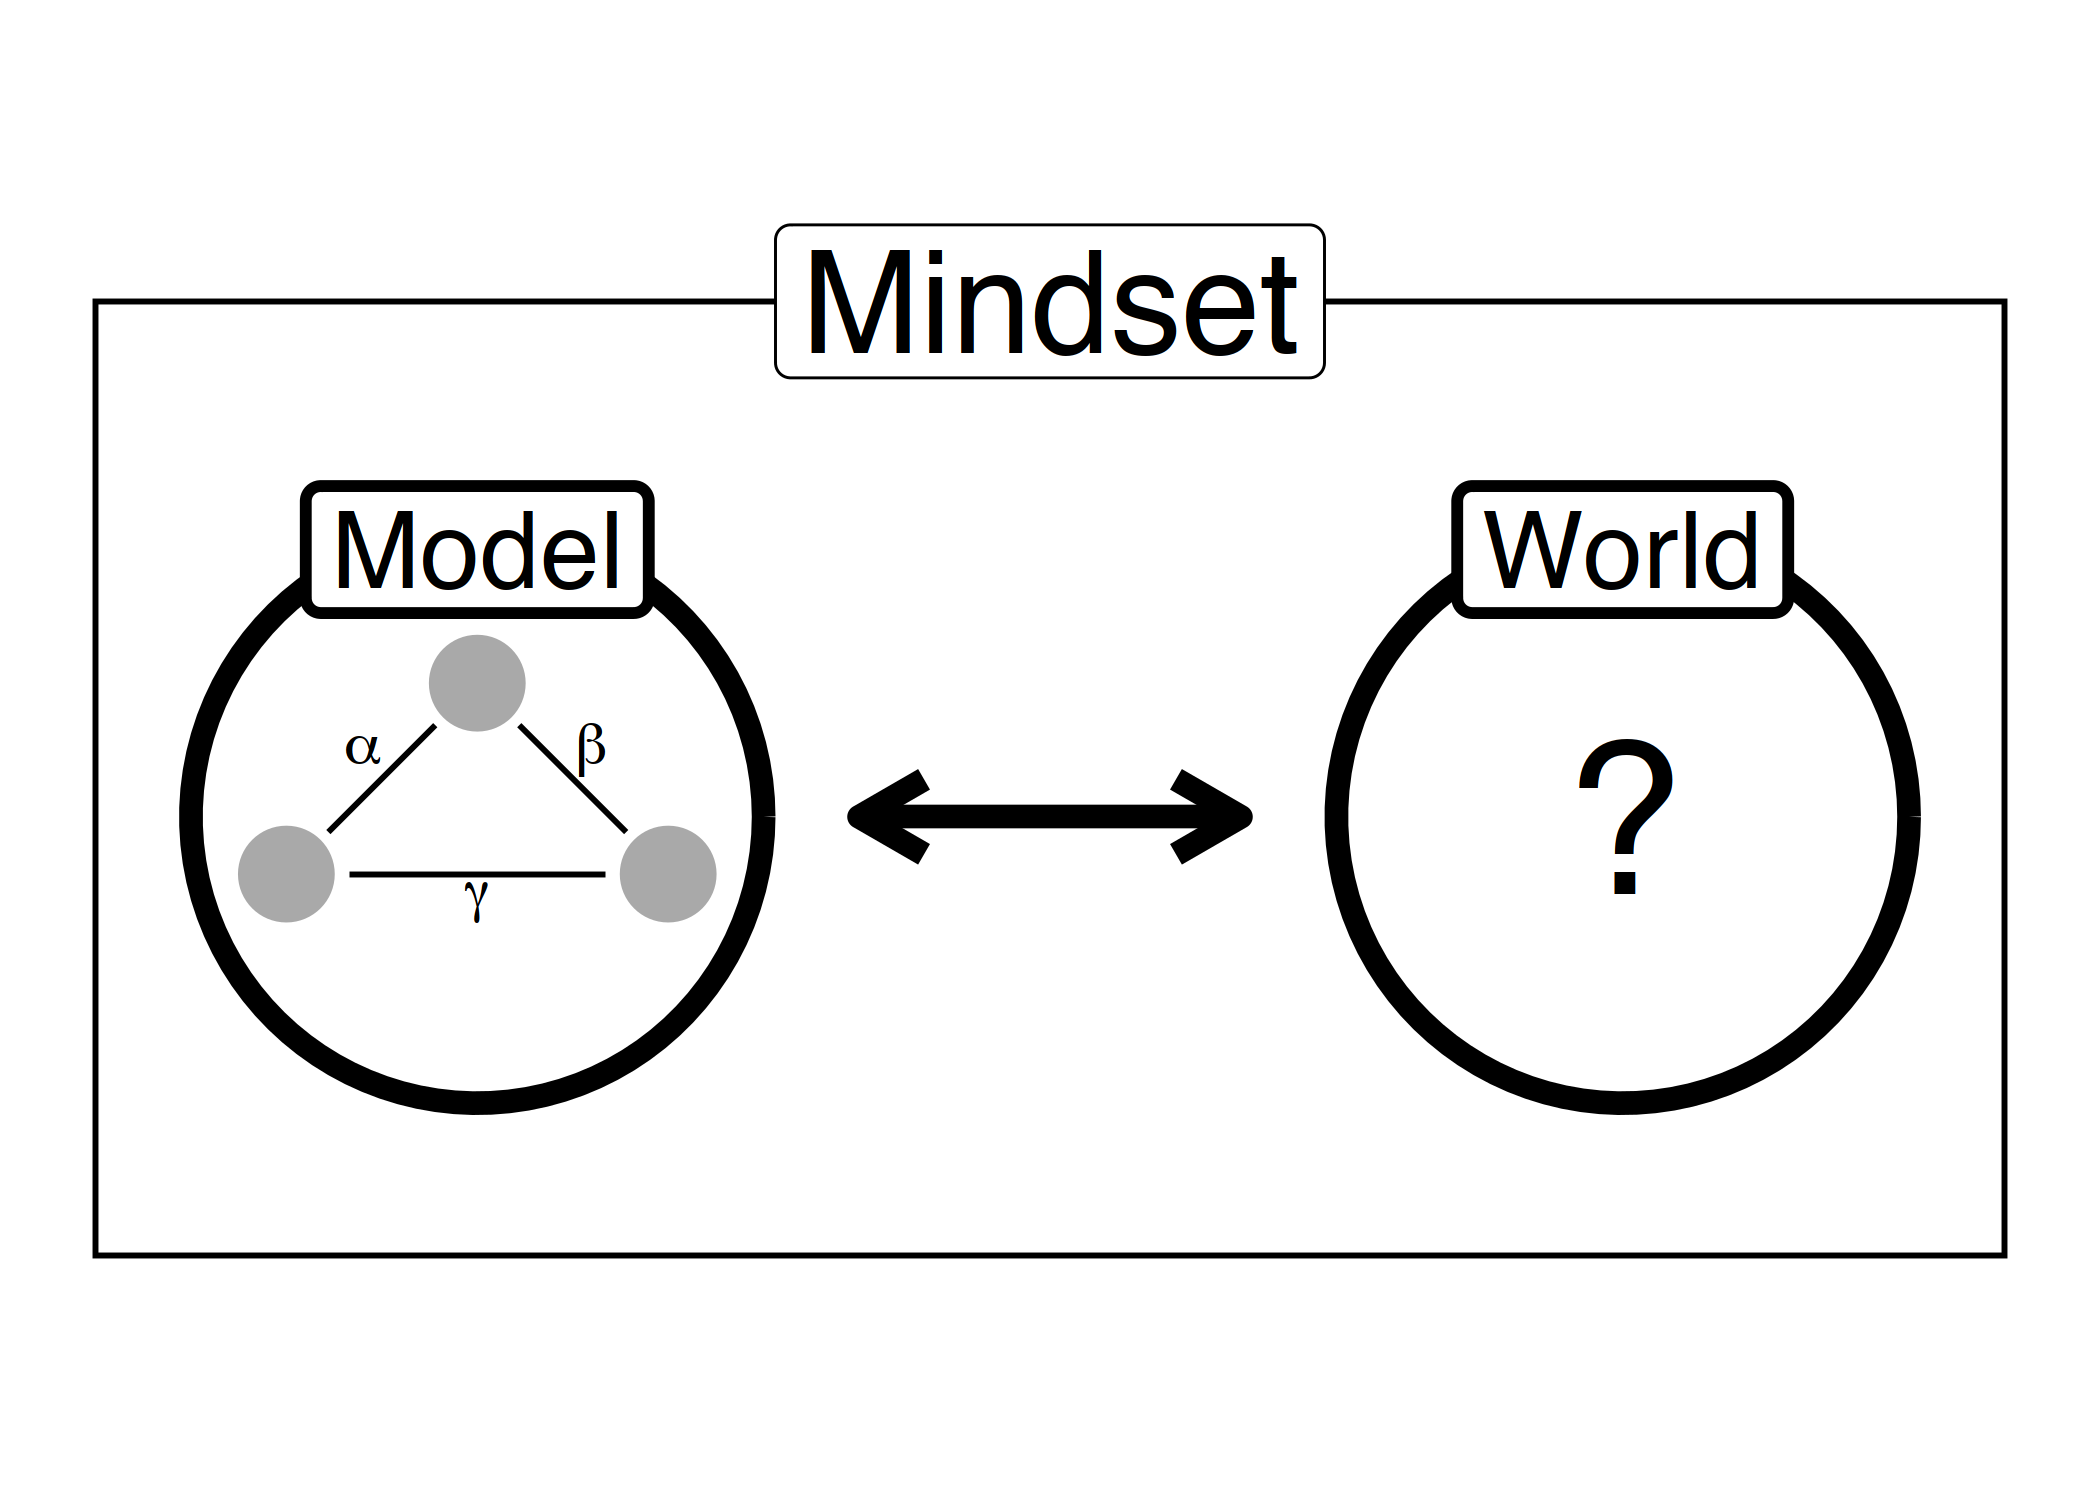
\includegraphics[width=0.8\textwidth]{figures/mindset-1} 

}

\caption{Only when a model is embedded in a mindset can we put it into context with the world.}\label{fig:mindset}
\end{figure}

\textbf{Modeling mindsets} are normative:
A modeling mindset distinguishes between good and bad models.
Even if model evaluations are partly based on objective criteria, the decision in favor of a criteria is subjective.
For a frequentist statistician, a good model of the world is probabilistic and has a high goodness-of-fit to the assumed distributions.
The residuals of the model also pass diagnostic checks.
The frequentist rejects the use of prior probabilities.
The frequentist would also not switch to a random forest just because it has a lower mean squared error on test data.
And why would the statistician switch?
From their point of view, the random forest is a poor model of the world.
We learn nothing about the probability distribution of our variables.
We can't do frequentist hypothesis testing of the effects of variables.
The performance of the frequentist's model on unseen test data is not as important to the frequentist.
Each mindset has their own set of accepted models and evaluation procedures.

A modeling mindset limits the questions that can be asked.
Consequently, some questions or tasks are out of scope of the mindset.
Often the questions are out of scope because they just don't make sense in a particular modeling mindset.
Supervised machine learners formulate tasks as prediction or classification problems.
Questions about probability distributions are out of reach since the mindset is: choose the model that has the lowest generalization error given new data.
So the best model could be any function, such as the average prediction of a random forest, a neural network, and a linear regression model.
If the best model can be any function, questions that a statistician would normally ask (hypothesis testing, parameter estimation, \ldots) become irrelevant to the machine learner.
In machine learning, the best models are usually not classical statistical models.
If the machine learner started asking questions a statistician would ask, they would have to choose a suboptimal model, which is a violation of the mindset.

\textbf{Modeling mindsets are cultural}.
Modeling mindsets are not just theories; they shape and are shaped by communities of people who model the world based on the mindset.
In many scientific communities, the frequentist mindset is very common.
I once consulted a medical student for his doctoral thesis.
I helped him visualize some data.
A few days later he came back, ``I need p-values with this visualization.''
His advisor told him that any data visualization needed p-values.
His advisor's advice was a bit extreme, and not advice that a real statistician would have given.
However, it serves as a good example of how a community perpetuates a certain mindset.
Likewise, if you were trying to publish a machine learning model in a journal that publishes mostly Bayesian analysis, I would wish you good luck.
And I'd bet 100 bucks that the paper would be rejected.

The people within a shared mindset also accept the assumptions of that mindset.
And these assumptions are usually not challenged, but mutually agreed upon, at least implicitly.
If you work in a team that has been using Bayesian statistics for some time, you won't be questioning each model anew about whether using priors is good or whether the Bayesian interpretation of probability is legit.
In machine learning competitions, the model with the lowest prediction error on new data wins.
You will have a hard time arguing that your model should have won because it's the only causal model.
If you believe that causality is important, you would simply not participate.
You can only thrive on those machine learning competition platform if you have accepted the supervised machine learning mindset.

The modeling mindsets as I present them in this book are archetypes: pure forms of these mindsets.
In reality, the boundaries between mindsets are much more fluid.
These archetypes of mindsets intermingle within individuals, communities and approaches:
A data scientist who primarily builds machine learning models might also use some simple regression models with hypothesis tests -- without cross-validating the models' generalization error.
A research community could accept analyses that use both frequentist and Bayesian statistics.
A machine learning competition could include a human jury who wards additional points if the model is interpretable and incorporates causal reasoning.

Have you ever met anyone who is really into supervised machine learning?
The first question they ask is ``Where is the labeled data?''.
The supervised machine learner turns every problem into a prediction or classification problem.
Or perhaps you've worked with a statistician who always wants to run hypothesis tests and regression models?
Or you had intense discussion about probability with a hardcore Bayesian?
Some people really are walking archetypes. 100\% of one archetype.
But I would say that most people learned one or two mindsets when they start out.
And later they got glimpses of other mindsets here and there.
Most people's mindset is already a mixture of multiple modeling mindsets.

\hypertarget{statistical-modeling}{%
\chapter{Statistical Modeling}\label{statistical-modeling}}

\begin{itemize}
\tightlist
\item
  Goal: Changing your mind under uncertainty.
\item
  Assumes the world is best described by probability distributions.
\item
  Statistical modeling fits probability distributions to data.
\item
  Requires further assumptions for drawing conclusions. See \protect\hyperlink{frequentism}{frequentism}, \protect\hyperlink{bayesian}{Bayesianism} and \protect\hyperlink{likelihoodism}{likelihoodism}.
\end{itemize}

Do you become more productive when you drink a lot of water?
Is there a fixed ``law'', like a mathematical function, that expresses productivity as a function of water intake?
No.
No, because productivity depends on many factors: sleep duration and quality, distractions, noise pollution, \ldots{}
Because of all these factors and other contingencies, we won't get a perfect equation relating water intake to productivity.
Uncertainty remains.
Even the water intake varies from day to day and from person to person.

Statistics is changing your mind under uncertainty.
One way to deal with the uncertainty of the world is to abstract aspects of the world as random variables and ascribe a probability distribution to them.
Daily water intake could be a random variable.
For productivity we would need some clever idea on how to best measure this abstract concept.
A not so clever example: Daily time spent in front of the computer.
To further relate these variables to each other, we can make assumptions on how the data were generated and connect the random variables in a statistical model.
Welcome to the statistical modeling mindset.

Statistical modeling is a parent to these other mindsets: \protect\hyperlink{frequentism}{frequentism}, \protect\hyperlink{bayesianism}{Bayesianism}, \protect\hyperlink{likelihoodism}{likelihoodism} and \protect\hyperlink{causality}{causal inference}.
These mindsets provide different ideas for how to do inference -- drawing conclusions about the world from data.
The mindsets differ in their interpretation of probability, their stance on causality and their faithfulness to the likelihood principle.
Their use of statistical models unites these mindsets.

A statistical model consists of a set of probability distributions.
A probability distribution describes the frequency with which we expect to see certain values of random variables.
The second ingredient to a statistical model is the data, from which we estimate those probability distributions.
Random variables are capture some aspect of the world.
But let's start with the most elementary unit: the random variable.

\hypertarget{random-variables}{%
\section{Random Variables}\label{random-variables}}

A random variable is a mathematical object that carries uncertainty.
Daily water intake can be a random variable.
Observed data are seen as \textbf{observations} or realizations of random variables.
If someone drank 2.5 liters of water, that is a realization of the random variable ``daily water intake''.

Other random variables:

\begin{itemize}
\tightlist
\item
  Outcome of a dice roll.
\item
  Monthly sales of an ice cream truck.
\item
  Whether or not a customer has canceled their contract last month.
\item
  Daily amount of rain in Europe.
\item
  Pain level of patients arriving at the emergency room.
\end{itemize}

People with a statistical modeling mindset \textbf{think} in random variables.
Any problem related to data is translated into a set of random variables and solved based on that representation.
A random variable is a construct that we can't observe directly.
But we can observe the realizations of a random variable, as shown in Figure \ref{fig:variable}.
But the raw data are not that useful to humans.
Because humans aren't databases, we need a model that simplifies the noisy data for us.
Statisticians came up with probability distributions: a mathematical construct that describes potential outcomes of the random variable.

\begin{figure}

{\centering 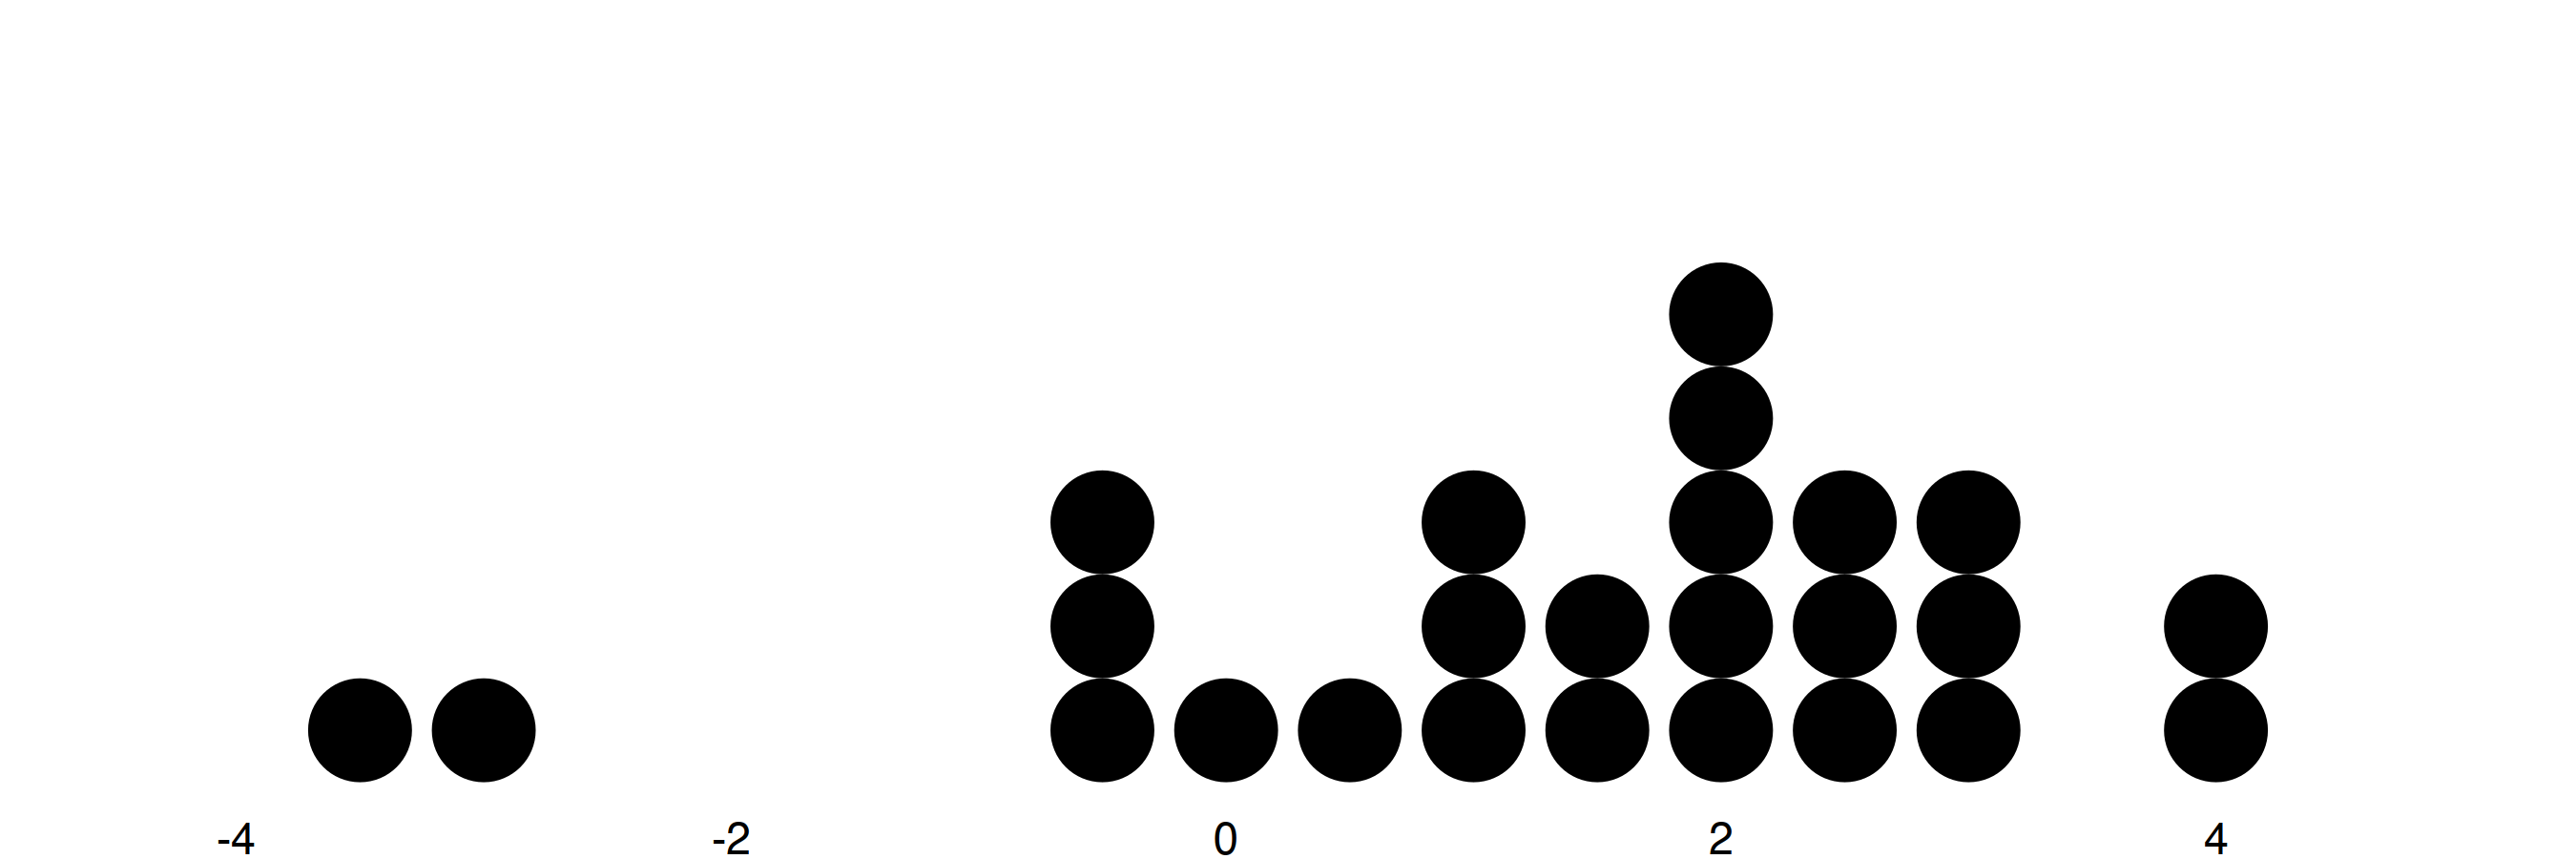
\includegraphics[width=0.8\textwidth]{figures/variable-1} 

}

\caption{Each dot represents a data point, a realizations of a random variable. The x-axis shows the value of the variable. Dots are stacked up for frequently occurring values. }\label{fig:variable}
\end{figure}

\hypertarget{probability-distributions}{%
\section{Probability Distributions}\label{probability-distributions}}

A probability distribution is a function which gives each possible outcome of a random variable a probability.
Value in, probability out. \footnote{For continuous variables like water intake, technically we may not interpret probability density functions at a certain value, like P(intake = 2.5 liter) as probability. Instead we have to take the integral, for example over the range of 2.4 to 2.6 liters and then may interpret as the probability.}
Not all functions can be used as probability functions.
A probability function must be larger or equal to zero for the entire range of the random variable.
For discrete variables such as the number of fish caught, the probability distribution must sum up to 1 over all possible outcomes.
And for continuous outcomes such as water intake, the probability distribution, also called density function, must integrate to 1 over the possible range of values.

For the outcome \(x\) of a fair dice, we can write the following probability function:

\[
P(x) = 
\begin{cases}
 1/6 & x \in \{1, \ldots, 6\} \\
 0 & x \notin \{1, \ldots, 6\} \\
\end{cases}
\]

The Normal distribution is for continuous variables and defined from minus to plus infinity:

\[f(x) = \frac{1}{\sigma \sqrt{2\pi}} e^{-\frac{1}{2}\left(\frac{x-\mu}{\sigma}\right)^2}\]

In this equation, \(\pi\) and \(e\) are the famous constants \(pi \approx 3.14\) and \(e \approx 2.7\).
The distribution has two parameters: mean \(mu\) and standard deviation \(\sigma\).

These parameters called location (\(\mu\)) and scale (\(\sigma\)) parameters, since they determine where on the x-axis the center of the Normal distribution is and how flat or sharp the distribution is.
The larger the standard deviation \(\sigma\), the flatter the distribution.

Let's try it out and set \(\mu = 0\) and \(\sigma = 1\), as visualized in Figure \ref{fig:distributions}, leftmost curve.
Now we can use this probability distribution function for telling us how probable certain values of our random variable are.
We get \(f(1) \approx 0.24\) and for \(f(2) \approx 0.05\), making \(x=1\) much more likely then \(x=2\).
We may not interpret \(f(x)\) as probability directly.
But we can integrate \(f\) over a region of the random variable to get a probability.
The probability for \(x \in [0.9, 1.1]\) is 4.8\%.

There is huge arsenal of probability distributions: The Normal distribution, the Binomial distribution, the Poisson distribution, \ldots{}
And there is an infinite number of probability distributions that you could invent yourself.

\begin{figure}

{\centering 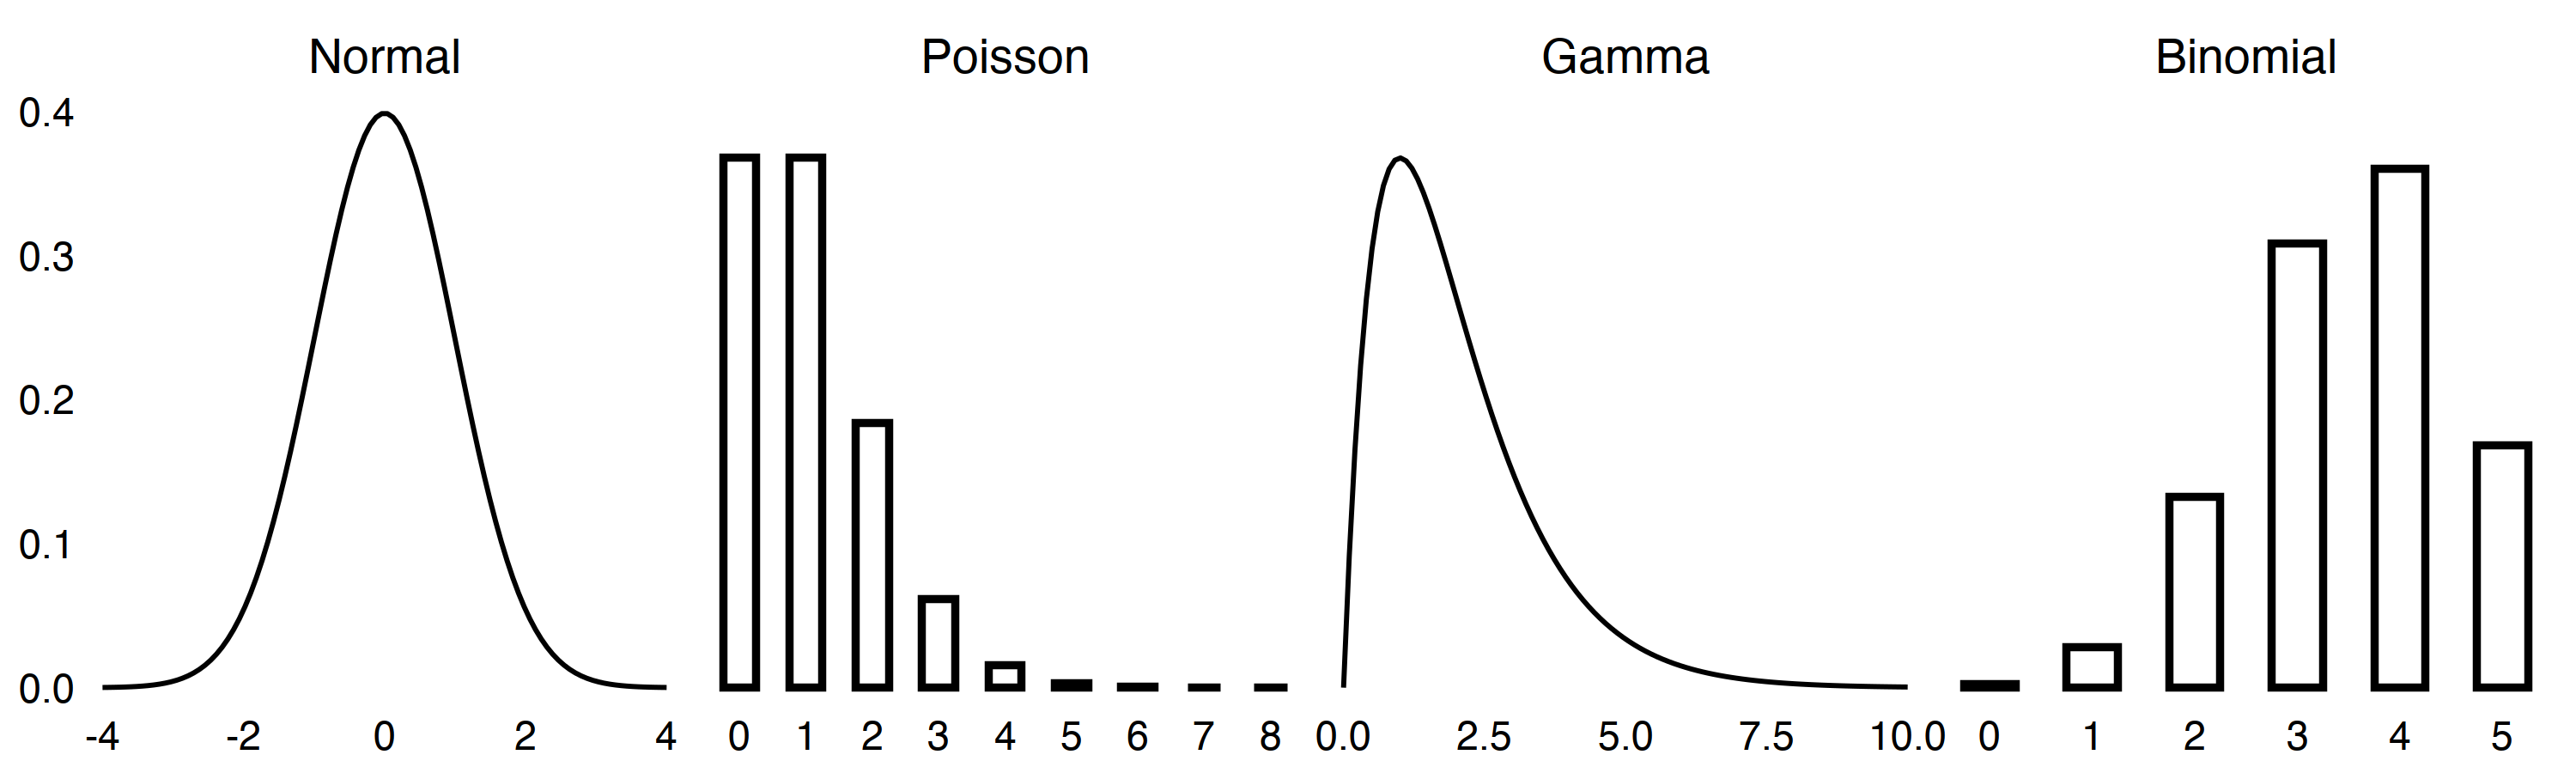
\includegraphics[width=0.8\textwidth]{figures/distributions-1} 

}

\caption{Distributions}\label{fig:distributions}
\end{figure}

\hypertarget{assuming-a-distribution}{%
\section{Assuming a Distribution}\label{assuming-a-distribution}}

An important step in the statistical modeling mindset is to connect the random variables that we are interested in to distributions.
A common approach is to choose a distribution that matches the ``nature'' of your data:

\begin{itemize}
\tightlist
\item
  A numerical outcome such as IQ? That's Normal distribution.
\item
  A count outcome, like number of fish caught per hour? The Poisson distribution is a solid choice.
\item
  A binary repeated outcome, like the number of successful free throws in basketball? It follows a Binomial distribution.
\end{itemize}

These were all examples of the distributions of single random variables.
The world is more complex than that:
Distributions of random variables can be intertwined.
The distribution of one variable can depend on the value that another random value takes on.
Fortunately, it's possible to define so-called multivariate distributions.
A multivariate distribution is a function that takes more than one value and returns a density (still a single number).
We might assume that the joint distribution of water intake and productivity (measured in minutes) follows a 2-dimensional Normal distribution.
Or we could assume that the productivity, conditional on water intake, follows a Normal distribution.
We can be very creative in defining distributions and so on.

With these probability distributions, we are still in the realm of abstraction and assumptions.
On one side we have the data: messy and untamed.
On the other side, we have the probability distributions: clean and idealized.
Statistician ideologically connect the two via random variables:
The data are the realizations of the random variables.
And the distributions summarize the stochastic behaviour of random variables.
But we still need to mathematically connect data and theoretical distributions.
How do we bring data and distributions together?

The answer is \textbf{statistical models}.

\hypertarget{statistical-model}{%
\section{Statistical Model}\label{statistical-model}}

A statistical model connects theoretical distributions with observed data.
Statistical models are mathematical models that make assumptions about how the data are generated, and are estimated using data.
More formally, a statistical model is the combination of the sample space from which the data comes from, and a set of probability distributions on this sample space.

The distributions are ``fitted'' to the data by changing the parameters.
Imagine the distribution as a cat.
And your data is a box.
Your cat fits it's shape and position to match the box.

How do we know which parameters to set in our distribution?
Here we can work with the probability distribution.
As I said, the probability distribution is a function that gives the probability or density, given the value of a data point.
And it's parameterized, for example by the mean and variance for the Normal distribution.
We can use the same function to also find our parameters -- by switching the point of view.
The likelihood function \(L(\theta | X)\) is the probability function, but seeing the parameters as changeable, and the data as fixed.
For each data point, we can compute the likelihood function.
And we can multiply these likelihoods, which gives us the likelihood for all of our data.
This is a function where we now can fill in some parameters, for example \(\mu = 1\) and \(\sigma = 2\) and get a value in return.
The larger the value, the better the distribution fits the data.

We have ourselves an optimization problem at hand: Maximize the likelihood function \(L\) with respect to the parameters, and given the data.
We want to maximize the likelihood for all of our data, so first we form the likelihood for our entire dataset \(L(\mathbf{x}_1, \ldots, \mathbf{x}_n) = \prod_{i=1}^n f(\mathbf{x}_i)\).
Emphasizing that \(\mathbf{x}_1\) can be a vector multiple variables, in this case for data point 1.
And we maximize the data likelihood:

\[\arg \max_{\theta} L(\theta | \mathbf{x}_1, \ldots, \mathbf{x}_n)\]

Maximum likelihood estimation is a classic optimization problem.
For simpler cases this can even be solved analytically, for example for the Normal distribution, we know that the ideal \(mu\) is the mean of the data: \(\frac{1}{n} \sum_{i=1}^n x_i\).
For likelihood maximization where the analytical solution is not possible, other optimization methods exists.

If you have understood the idea of maximum likelihood, you understand a key element the statistical modeling mindset.
Maximizing the likelihood means bringing together the theoretical probability distributions and the observed data.
We fit the distributions, aka our statistical model, to the data.

\begin{figure}

{\centering 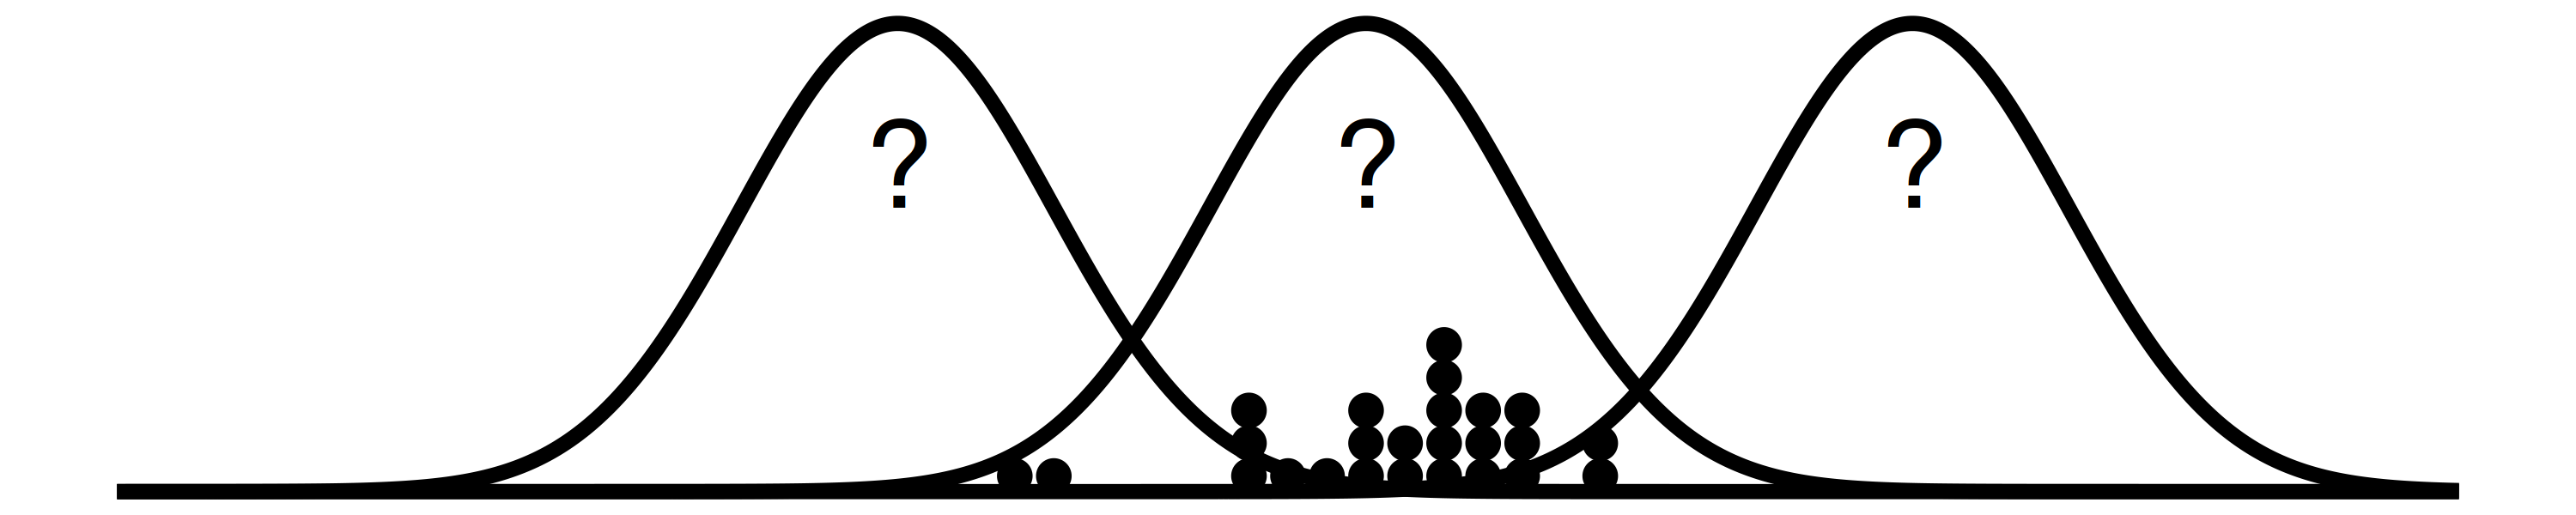
\includegraphics[width=0.8\textwidth]{figures/fit-1} 

}

\caption{Fitting distributions to data}\label{fig:fit}
\end{figure}

The role of the distribution parameters goes well beyond a technical one.
The parameters are central to the statistical modeling mindset.
We can interpret the parameters as summarization of our data!
Statistical modeling is about understanding our data better.
The nice consequence of modeling our data with probability distributions is that we summarize our data with a few numbers, the parameters.
In the case of the Gaussian distribution, we can describe the distribution of a single variable with only two numbers, the mean and the standard deviation.
Also for other types of statistical models, parameters are central to interpretation.

\hypertarget{types-of-statistical-models}{%
\section{Types of Statistical Models}\label{types-of-statistical-models}}

All statistical models target an aspect of a probability distribution.
For most of the chapter, we talked about simpler cases, like having the distribution of a single variable and fitting a distribution.
So the case was of learning \(P(X)\).
But we could have the case of multiple random variables \(X_1, \ldots, X_p\).

We have two options (bit oversimplifying here) for the probability distribution:
Fit the joint distribution, or a conditional distribution.
Depending on the problem that we want to solve, there are different properties of the distribution that we might want to find out.
Very often, it's a conditional mean: ``What do we expect for a random variable \(Y\) given \(X= \mathbf{x}\)?
But it can also be other parts of the distribution:''What's the 90\% quantile for \(Y\) given \(X = \mathbf{x}\)?
Consequently, 10\% of the values for \(Y\), given \(X=\mathbf{x}\), would be greater than the 90\% quantile.
Think of insurance: An insurance company is noy only interested in the expected damages they have to cover, but also how much they would have to cover in the extreme case.

A Gaussian mixture model, for example, requires learning the entire distribution.
Gaussian mixture models can be used for identifying clusters in the data, which are assumed to stem from a mixture of Normal distributions.
With Gaussian mixture models we also seen an example where maximum likelihood is not the sole optimization approach.
Instead, the expectation-maximization algorithm is used, which iteratively jumps between optimizing the model parameters and predicting the ``mixture'' of cluster centers for each data point.

The joint distribution is not always of interest.
So often, the modeler is only interested in the conditional distribution:
How does the probability distribution of a variable depend on other variables?
For example:

\begin{itemize}
\tightlist
\item
  What are risk factors that influence the probability of getting lung cancer?
\item
  How do climatic conditions like temperature and humidity affect the occurence of bonobos?
\item
  On which days is a hospital likely to be understaffed?
\end{itemize}

The conditional distribution is the natural form for prediction tasks and usually simpler to estimate than the joint distribution.
Models of the conditional distribution are central to statistical modeling.
They are also known as regression models.

\hypertarget{regression-models}{%
\section{Regression Models}\label{regression-models}}

Regression models are statistical models that don't learn the joint distribution, but a conditional distribution.
Let's say we have two variables: \(Y\) and \(X\).
With the join distribution \(P(Y,X)\) we could answer ``How likely is a certain combination of \(X=x\), and \(Y=y\).
But with the joint distribution, we can ask:''Given \(X=x\), what is the probability distribution of \(Y\)``?

For example, we want to know not only how often a disease is successfully treated.
We might want to know if a certain drug played a part in the disease outcome.
And other factors such as age of the patient, progression of the disease and so on might play a role as well.
And we would have to consider such factors to answer the question on whether the drug helps.

Our target is the distribution of outcome variable \(Y\) conditionanl on variables \(X_1, \ldots, X_p\).
That means that within the regression model the parameters of the distribution of \(Y\) are linked to the other variables.
How exactly this link looks like depends on the distribution that the modeler assumed for \(Y\) and the link they chose to connect the two.
The simplest case is a linear model.
We assume that \(Y\) follows a Normal distribution and link the mean of \(Y\)'s distribution to a weighted sum of the other variables:

\[Y \sim N(\mu, \sigma)\]

\[\mu = \beta_0 + \beta_1 X_1 + \ldots + \beta_p X_p\]

The linear regression model expresses the mean of the target \(Y\) as the weighted sum of the other variables.
\(Y\) given \(\mathbf{X}\) follows a Normal distribution.
We only link the mean \(\mu\) to the variables.
A typical assumption is that the \(\sigma\) is independent of the value of the other variables.

What can we do now with a regression model?
We can make predictions.
We just have to fill in values for \(X\) and get the expected value of the probability distribution of \(X\).
Another typical goal is interpreting the relationship between the target with the other variables.
The coefficients in the regression model are subject to interpretation.
For the linear regression model, a positive coefficient \(\beta_j\) means that increasing the value of variable \(X_j\) increases the expected value of \(Y\).

Thinking in regression models brings you closer to the \protect\hyperlink{mindset}{supervised machine learning}.
However, in supervised machine learning, the focus is usually on getting a good predictive model.
Not on finding a finding a probabilistic representation of your data with random variables and distributions.

But what if the outcome is a category, and our task is classification?
When you come from the \protect\hyperlink{supervised-ml}{supervised machine learning} mindset, always the distinction between classification and regression models is made.
In statistical modeling, we don't model the categories, but their probability distribution.
From the statistical modeling mindset, a categorical variable is nothing special.
Like for all other variables, we model the conditional distribution of the variable.
And if we make predictions with our model, we get the probabilities for the categories.

\hypertarget{model-evaluation}{%
\section{Model Evaluation}\label{model-evaluation}}

Statistical models can be evaluated.
The evaluation is very revealing to understand the mindset.
And especially how the statistical modeling mindset differs from the \protect\hyperlink{supervised-ml}{supervised machine learning} mindset.
Evaluation consists of model diagnostics and goodness-of-fit measures.

The role of model diagnostics is to check whether the modeling assumptions were meaningful.
If we assumed that a random variable follows a Normal distribution, we can visually check whether that's really the case using, for example, the Q-Q plot.
An assumption for linear regression model that I mentioned : The variance of the outcome does not depend on the values of the other variables.
This can be checked visually by plotting the residuals (value of \(Y\) minus predicted value of \(Y\)) against each of the other variables.

The role of goodness-of-fit measures is model comparison and evaluating modeling choices.
Typical measures here are the (adjusted) R-squared, Akaikes Information Criterion (AIC), the Bayes factor, and likelihood ratios.
Goodness-of-fit are, quite literally, measures that tell us how well our model fits the data.
Goodness-of-fit metrics can guide the model building process and decide which model to choose in the end.

Goodness-of-fit metrics are typically computed with the same data that were used for fitting the statistical models.
This choice may look like a minor detail, but it says a lot about the statistical modeling mindset.
The critical factor here is overfitting: The more flexible a model is, the better it adapts to ALL the randomness in the data instead of learning patterns that generalize.
Many goodness-of-fit metrics therefore account for model complexity, like the AIC or adjusted R-squared.
For the \protect\hyperlink{supervised-ml}{supervised machine learning} mindset, you would always use new, unseen data for the evaluation.

\hypertarget{data-generating-process-dgp}{%
\section{Data-Generating Process (DGP)}\label{data-generating-process-dgp}}

A quite central, but fuzzy topic of the statistical modeling mindset is the data-generating process.
The statistical modeler thinks about the data-generating process all the time.
The data-generating process is a construct, an unknowable ideal of how the data was generated.
The data-generating process produces the unknown distributions that than produce the data.
We can only observe the data-generating indirectly by oberving data.
And we can come closer to the DGP by reasoning about it.
You won't find this in any statistics book explicitly.
But it's the mindset of statistical modeling to have this idea of the DGP.
It's a natural consequence when you think about the world as random variables and distributions.

I think the DGP is a very powerful idea, even when it's not well defined.
Assuming a DGP encourages you to intellectually dive deep into your data.
Having this image of a DGP in your mind let's you take on the mindset of a detective:
Statisticians are like detectives reconstructing a crime.
You can't observe the crime directly.
But the crime has generated a lot of ``data'' at the scene.
The stats detective then tries to uncover the data-generating process by making assumptions and learning from data.

``Defining'' the data-generating process is neither simple nor well-defined, but I'll give it a try:

\begin{itemize}
\tightlist
\item
  Dice roll: the throw of the dice is the data-generating process. The dice is symmetric, which makes each side equally likely. We could factor in throwing angle, surface roughness and so on, but the chaotic behaviour of the dice jumping and spinning over the table makes us dismiss all these factors.
\item
  We study the income of computer scientists via a survey. Instead of only reporting on the income distribution, we think about the entire data-generating process: For example, some income values are missing. Are they missing at random? Or are maybe people with higher incomes omitting the question? Are some companies overrepresentated in the survey? Is the sample truly random?
\item
  A research team has collected chest x-ray images of patients with and without COVID-19 for building a COVID-19 prediction model. A closer look at the data-generating proces shows: the images not only differ in COVID-19 status, but they come from different data-generating processes. COVID-19 images are more likely from a horizontal position where the patient lies down because they are so exhausted. One of the non-COVID-19 datasets are even just children x-ray images. \footnote{Wynants, Laure, Ben Van Calster, Gary S. Collins, Richard D. Riley, Georg Heinze, Ewoud Schuit, Marc MJ Bonten et al.~``Prediction models for diagnosis and prognosis of covid-19: systematic review and critical appraisal.'' bmj 369 (2020).} I picked this example, because it is a paper from a \protect\hyperlink{machine-learning}{machine learning mindset}. Statisticians would think much more about the data-generating process, and are, IMHO, more likely to spot such mistakes.
\end{itemize}

If these examples of data-generating process sound like common sense to you, it's because they are.
But it's surprisingly uncommon among non-statistician mindsets.
For example, for \protect\hyperlink{machine-learning}{machine learning} considerations of the data-generating process play a subordinate .
For machine learning competitions, for example, the winner is, most of the times, solely determined by the lowest loss function.
It's not considered when some approach has a more meaningful consideration of the data-generating process, and an understandable model.

Sometimes we want to control at least parts of the data-generating process.
In randomized clinical trials, for example, we control who gets the drug and who get the placebo.
In other controlled experiments we even control more factors.

\hypertarget{drawing-conclusions-about-the-world}{%
\section{Drawing Conclusions About the World}\label{drawing-conclusions-about-the-world}}

Statisticians collect data about the world and use that data to fit a statistical model.
The statistical model links the world and the data through random variables:
The world can be simplified by probability distributions;
the data are viewed as realizations of the random variables.

Statistical modeling is a practical endeavour.
In most cases, statistical models are built for practical reasons:
To make a decision, to better understand some property of the world, or to make a prediction.
These goals requires us to interpret the model instead of the world.
But this interpretation does not come for free.
After all the model building and evaluation, the statistical modeler must consider the representativeness of the data, the interpretation of probability and causality.

Considering the data-generating process also means thinking about the representativeness of the data, and thus the model.
Are the data a good sample and representative of the quantity of the world you are interested in?
Let's say a statistical modeler analyzes data on whether a sepsis screening tool successfully reduced the incidence of sepsis in a hospital.
They conclude that the sepsis screening tool has helped reduce sepsis-related deaths at that hospital.
Are the data representative of all hospitals in the region, the country, or even the world?
Are the data even representative of all patients at the hospital, or are data only available from patients in intensive care unit?
In the statistical modeling mindset, defining the ``population'' from which the data are a sample and discussing how representative the data are of that population is critical to any conclusions drawn from the model.
\protect\hyperlink{design-based}{Design-based inference} fully embraces this mindset that the data are sampled from a larger population.

More philosophical is the modeler's attitude to causality, prior probabilities and the likelihood principle.
And, more general, how probability is to be interpreted.

\begin{quote}
``It is unanimously agreed that statistics depends somehow on probability. But, as to what probability is and how it is connected with statistics, there has seldom been such complete disagreement and breakdown of communication since the Tower of Babel.''
\end{quote}

-- Leonard Savage, 1972 \footnote{Savage, Leonard J. The foundations of statistics. Courier Corporation, 1972.}

Statistical modeling is the foundation for learning from data.
But we need another mindset on top of that to make the models useful.

\protect\hyperlink{frequentism}{Frequentist inference} is the most prominent mindset for inferring properties about the world from statistical models.
Frequentist statistics sees probability as the relative frequencies of events in long-run experiments.

\protect\hyperlink{bayesian}{Bayesian inference} is based on an interpretation of probability as a degree belief about the world.
Bayesianism states that the model parameters also have a (prior) distribution.
And the goal of the statistician is to update the prior distribution by learning from data.
The resulting posteriori distribution of the parameter expresses our belief about the the parameter.

\protect\hyperlink{likelihoodism}{Likelihoodism} is a lesser known modeling mindset. Like Bayesianism, it adheres to the likelihood principle, which states that the likelihood function captures all evidence from the data (which frequentist inference violates).
However, it does not require prior probabilities.

\protect\hyperlink{causality}{Causal inference} adds causality to statistical modeling. It can be superimposed onto any of the other three mindsets.

A different but complimentary approach is \protect\hyperlink{design}{design-based inference}, which focuses on data sampling and experiments instead of models.

\hypertarget{strengths}{%
\section{Strengths}\label{strengths}}

\begin{itemize}
\tightlist
\item
  The statistical modeling mindset is a \emph{language to see the world}. Even when not used for inference, random variables and probability distributions are useful mental models for perceiving the world.
\item
  Statistical modeling has a long tradition and extensive theoretical foundation, from measurement theory as the basis of probability theory to convergence properties of statistical estimators.
\item
  The data-generating process is an underestimated mental model. But it's a powerful mental model that encourages mindful modeling and asking the right questions.
\item
  Conditional probability models can be used not only to learn about the parameters of interest, but also to make predictions
\item
  Probability distributions give us a language to express uncertainty. \protect\hyperlink{bayesianism}{Bayesianism} arguably has the most principled focus on formalizing and modeling uncertainty.
\end{itemize}

\hypertarget{limitations}{%
\section{Limitations}\label{limitations}}

\begin{itemize}
\tightlist
\item
  Statistical modeling quickly reaches its limits when defining probability distributions becomes difficult. Images and text don't easily fit into this mindset, and this where \protect\hyperlink{supervised-ml}{supervised machine learning} and especially \protect\hyperlink{deep-learning}{deep learning} shine.
\item
  Working with the statistical modeling mindset can be quite ``manual'' and tedious. It's not easy to always think about the DGP, and sometimes more automatable mindsets such as supervised machine learning are more convenient.
\item
  Statistical models require a lot of assumptions. Sometimes more, sometimes less. Just to name a few common assumptions: homoscedasticity, independent and identically distributed data (IID), linearity, independence of errors, lack of (perfect) multicollinearity, \ldots{} For most violations, there is a special version of a statistical model without the critical assumption whose estimation and interpretation is often more complicated.
\item
  Statistical modeling, when used for prediction, is often outperformed by \protect\hyperlink{supervised-ml}{supervised machine learning}. To be fair, outperforming here requires an evaluation based on the supervised learning mindset. However, this means that a goodness-of-fit and diagnostics are no guarantee that a model will performs well on all metrics.
\end{itemize}

\hypertarget{statistical-inference}{%
\chapter{Frequentist Inference}\label{statistical-inference}}

\begin{itemize}
\tightlist
\item
  The most popular modeling mindset for scientific questions.
\item
  The world consists of probability distributions with fixed parameters that have to be uncovered.
\item
  Interprets probability as long-run relative frequencies from which hypothesis tests, confidence intervals and p-values are derived.
\item
  A statistical mindset, with \protect\hyperlink{bayesian}{Bayesian inference} and \protect\hyperlink{likelihoodism}{likelihoodism} as alternatives.
\end{itemize}

Drinking alcohol is associated with a higher risk of diabetes in middle-aged men.
At least this is what a study claims \footnote{Kao, WH Linda, Ian B. Puddey, Lori L. Boland, Robert L. Watson, and Frederick L. Brancati. ``Alcohol consumption and the risk of type 2 diabetes mellitus: atherosclerosis risk in communities study.'' American journal of epidemiology 154, no. 8 (2001): 748-757.}.
The study modeled type II diabetes risk as a function of various risk factors.
The researchers found out that alcohol significantly increases the diabetes risk by a factor of \(1.81\).

``Significant'' and ``associated with'' are familiar terms when reading about scientific results.
The researchers in the study used a popular modeling mindset to draw conclusions from the data: frequentist inference.
There is no particular reason why I chose this study other than it is not exceptional.
When someone thinks in significance levels, p-values, hypothesis tests, null hypotheses, and confidence intervals, they are probably frequentist.

In many scientific fields, such as medicine and psychology, frequentist inference is the dominant mindset.
All frequentist scientific papers follow similar patterns, make similar assumptions, and contain similar tables and figures.
Knowing how to interpret model coefficients, confidence intervals and p-values is like a key to contemporary scientific progress.
Or at least a good part of it.
Frequentism not only dominates science, but has a firm foothold in industry as well:
Statistician, data scientists, and whatever the role will be called in the future, use frequentist inference to create value to their businesses:
From analyzing A/B tests for website to calculating portfolio risk to monitoring quality on production lines.

As much as frequentism dominates the world of data, it's also criticized.
Frequentist inference has been the analysis method for scientific ``findings'' that turned out to be a waste of research time.
You may have heard about the replication crisis. \footnote{Ioannidis, John PA. ``Why most published research findings are false.'' PLoS medicine 2, no. 8 (2005): e124.}
Many scientific findings in psychology, medicine, social sciences and other fields could not be replicated.
The problem is that replication is at the center of the scientific method.
While many causes have contributed to the replication crisis, frequentist statistics is right in the middle of it.
The frequentist mindset enables practices such as multiple testing and p-hacking.
Mix this with the pressure on academics to ``publish or perish'', and an entire community is incentivized to squeeze out ``significant'' results.
Frequentism is a decision-focused mindset and can give seemingly simple yes/no answers.
Lazy as most of us are, we then tend to forget all the footnotes and remarks that come with the model.

Frequentist inference is a statistical modeling mindset.
As such, it depends on random variables, probability distributions, and statistical models.
But as mentioned in the chapter \protect\hyperlink{statistical-modeling}{Statistical Modeling}, these ingredients are not sufficient to make statements about the world.

Frequentism comes with a specific interpretation of probability:
Probability is seen as the relative frequency of an event in infinitely repeated trials.
That's why it's called frequentism: frequentist inference emphasizes the (relative) frequency of events.
But how do these long-run frequencies help to gain insights from the model?

Let's go back to the \(1.81\) increase in diabetes risk among men who drink a lot of alcohol.
\(1.81\) is larger more than \(1\), so there seems to be a difference between men who drink alcohol and the ones who don't.
But how can the researchers be sure that the \(1.81\) is not a random result?
For fair dice, the average eyes in the long run series of experiments is 3.5.
If I roll a die 10 times and the average is 4, would you say it's an unfair die?
No? Would you say it's unfair if the average is 4.5? 5? Or if a 6 shows up 10 times?

The researchers applied frequentist thinking to decide between randomness and true effects.
The parameter of interest is a coefficient in a logistic regression model.
The logistic regression model links variables such as alcohol intake to the occurrence of diabetes.
In the diabetes study, a 95\% confidence interval for the alcohol coefficient is reported from \(1.14\) to \(2.92\).
This interval settles the question of randomness versus signal:
The interval doesn't contain \(1\), and so the researchers concluded that alcohol is a risk factor for diabetes (in men).
This confidence interval describes uncertainty regarding the alcohol coefficient.
If we were to repeat the experiment, including the modeling, many times, the respective 95\% confidence interval would cover the ``true'' parameter 95\% of the time.
Always with the footnote that the model assumptions were correct.

\hypertarget{frequentist-probability}{%
\section{Frequentist probability}\label{frequentist-probability}}

The interpretation of the confidence interval reveals the core philosophy of frequentism:
The world can be described by probability distributions;
The parameters of the probability distributions are constant and unknown;
Repeated measurements/experiments reveal the true parameter values in the long-run.
In contrast, \protect\hyperlink{bayesian}{Bayesianism} assumes that the parameters of the distributions are themselves random variables.
As the frequentists collect more and more data (\(n \to \infty\)), their parameter estimators gets closer and closer to the true parameter (if the estimator is unbiased).
With each additional data point, the uncertainty of the estimated parameter shrinks and the confidence interval becomes narrower.

The frequentist interpretation of probability requires imagination.
Frequentists start with a population in mind.
The population can be adults between 20 and 29 living in Iceland, daily measurements of water quality of the Nile River, or 1-inch wood screws manufactured in a factory in U.S. state of Texas.
These populations can be described by finding out their probability distributions.
Going back to the initial example:
What's the probability that a middle-aged man will develop diabetes in the next 12 months?
Frequentists would say: There is an unknown and fixed probability for diabetes.
The more people we observe, the more accurate our estimate of the probability of diabetes becomes.
We estimate the probability of diabetes as the relative frequency of diabetes in the population.
Probabilities are frequencies in the long run: \(P(X=1) = \lim_{n \mapsto \infty} \frac{\sum_{i=1}^{n} I(x_i = 1)}{n}\).

\begin{figure}

{\centering 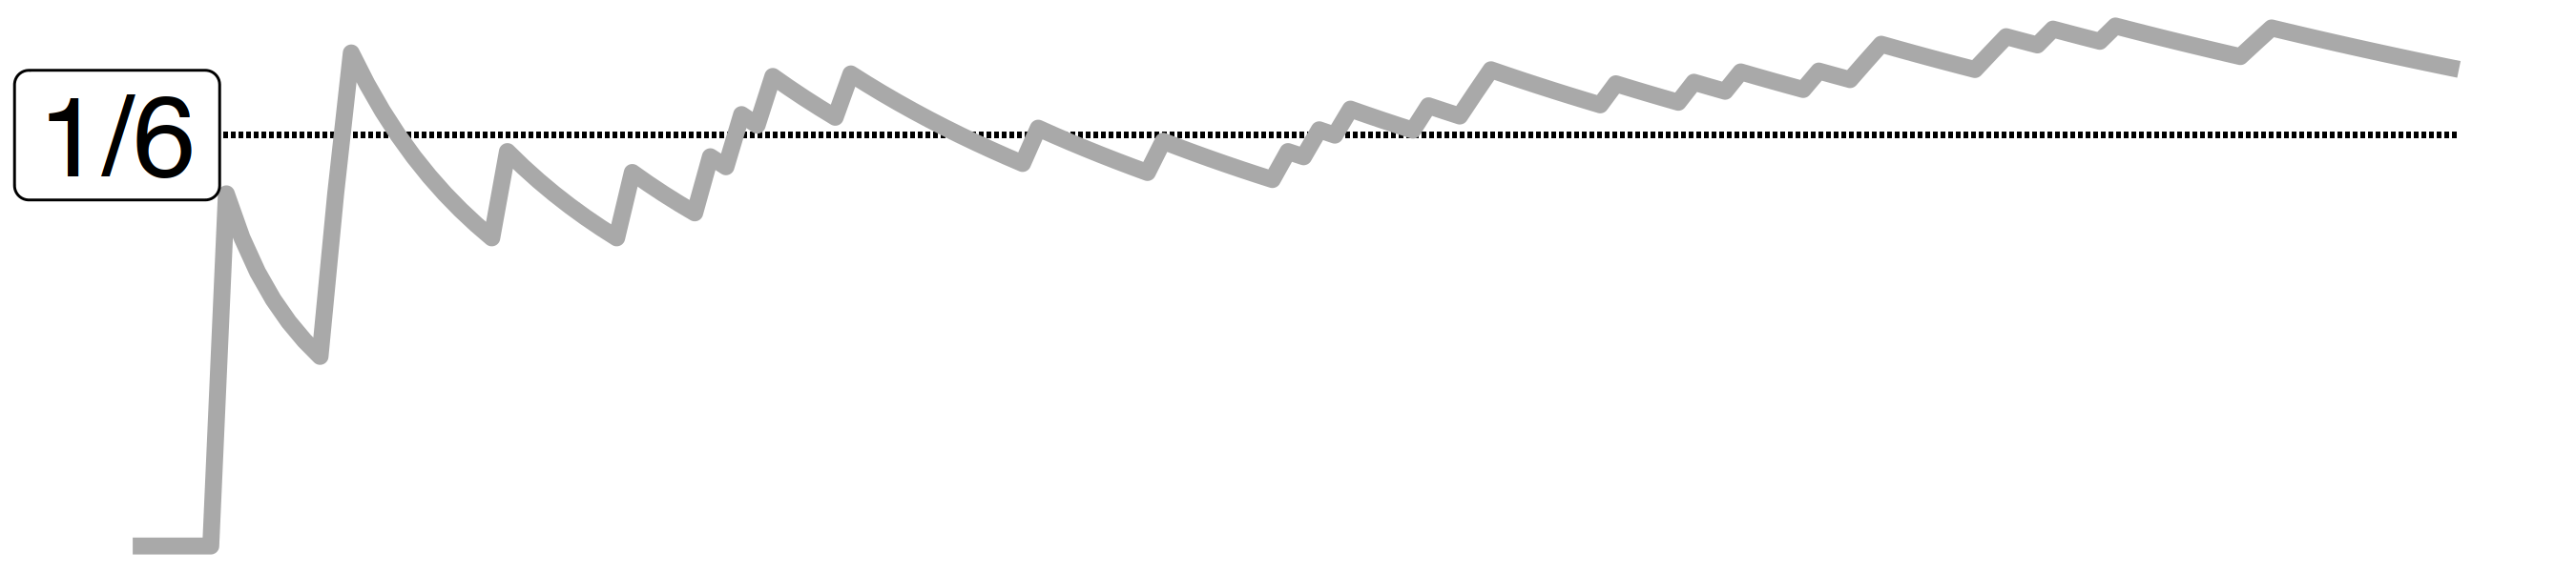
\includegraphics[width=0.8\textwidth]{figures/dice-1} 

}

\caption{The line shows how the relative frequency of 6 eyes changes as the number of dice roles increases from 1 to 100 (left to right).}\label{fig:dice}
\end{figure}

Imagining experiments that will never take place is essential to the frequentist mindset.
By defining probability in terms of long-run frequencies, the entire mindset requires imagining that the sampling and experiment will be done many times.
These ``imagined'' experiments are central to the interpretation of confidence intervals, p-values, and hypothesis tests.

These imagined experiments have a curious implication for frequentism.
Frequentism violates the likelihood principle, which says that all evidence about the data is contained in the likelihood function.
But with frequentism, it's important to know what experiments we are further imagining.
You can find a simple example involving coin tosses in the \protect\hyperlink{likelihoodism}{Likelihoodism chapter}.
In contrast, both \protect\hyperlink{likelihoodism}{Likelihoodism} and \protect\hyperlink{bayesianism}{Bayesianism} adhere to the likelihood principle.

\hypertarget{estimators-are-random-variables}{%
\section{Estimators are Random Variables}\label{estimators-are-random-variables}}

We can learn a lot about frequentist inference, especially in contrast to Bayesian inference, by understanding which ``things'' are random variables and which are not.
In the frequentist mindset, the estimand, the ``true'' but unknown parameter is assumed to be fixed.
Mean, variance and other distribution parameters, model coefficients, nuisance parameters, all are seen as having some unknown but fixed value.
And the values can be uncovered with frequentist inference.
Bayesians, in contrast, view all these parameter as random variables.

Since the quantities of interest are seen as fixed but unkown, the frequentist's job is to estimate them from data.
The estimation is done with a statistical estimator: A mathematical procedure for inferring the estimand from data.
The estimator is a function of the data.
And data are realizations of random variables.
The consequence is that also the estimators themselves are random variables.
Again, we can contrast this with Bayesian mindset:
Bayesians assume that the parameters are random variables.
Bayesians simply update the (prior) probability distribution of the parameters and get new (posterior) probability distributions.

Typical frequentist constructs like confidence intervals, test statistics and p-values are also random variables.
Mix this with the long-run frequencies and you get a special interpretation, for example, for \protect\hyperlink{confidence-intervals}{confidence intervals}.

Let's say you want to know how many teas you drink on average per day.
If you were frequentist, you would assume that there is a true but unknown average number of teas.
Let's call this estimand \(\lambda\).
The frequentist might assume that the daily number of teas follows a Poisson distribution.
The Poisson distribution can handle count data well, and is described by the ``intensity'' \(\lambda\) with which events happen.
Conveniently, the intensity parameter \(\lambda\) is also the expected number of events.
Teas in our case.
We could estimate the tea intensity using the maximum likelihood estimator: \(\hat{\lambda}= \frac{1}{n} \sum_{i=1}^n k_i\), where \(k_i\) is the number of teas on day \(i\).
Our estimator \(\hat{\lambda}\) is a random variable.
If the model assumptions are correct and if the world is truly frequentist, then the estimator \(\hat{\lambda}\) will get closer and closer to the true \(\lambda\) as \(n\) increases.
\(\hat{\lambda}\) approximately follows a Normal distribution.

Frequentist inference builds on the fact that the estimators are random variables.
Combined with the idea of fixed true parameters, it becomes possible to connect the analysis results to the real world.
A commonly used tool to derive insights about the world is null hypothesis significance testing.

\hypertarget{null-hypothesis-significance-testing}{%
\section{Null Hypothesis Significance Testing}\label{null-hypothesis-significance-testing}}

Let's say, your estimator \(\hat{\lambda}\) says that you drink 2.5 teas per month on average.
Initially you had the hypothesis that you drink 3.0 teas per month.
Obviously \(2.5 \neq 3.0\), so the initial hypothesis is incorrect.
Case closed.
But that would be too simple an answer, wouldn't it?
You also wouldn't say that a coin is unfair if heads come up in 51/100 tosses just because \(51 \neq 50\).
But when would a frequentist reject the initial hypothesis of 3.0 teas?
Would we reject the hypothesis if we get \(\hat{\lambda}<2.9\), or \(\hat{\lambda}<2.5\) or maybe must it be much lower, like \(\hat{\lambda}<1.5\)?
Only with the \protect\hyperlink{statistical-modeling}{statistical modeling mindset} we can't answer this question.

The frequentist mindset has an answer to this question of whether to accept or reject a hypothesis.
The frequentist estimator for the number of teas is a random variable that is supposed to approximate the true number of teas.
We can make (frequentist) probabilistic statements about this estimator.
And while the true value for \(\lambda\) is unknown, we can study the hypothesis of \(\lambda = 3.0\) by examining the random variable \(\hat{\lambda}\).

This idea of proposing a hypothesis, and then accepting or rejecting it based on a statistical model or test is called null hypothesis significance testing.
Hypothesis testing is a central method in the frequentist modeling mindset.
Hypothesis tests simplify decisions:
The frequentist accepts or rejects the so-called null hypothesis based on the results of the statistical model.
A statistical model can be very simple:
It can be as simple as assuming that the data follow a Normal distribution and comparing two means with a Student t-test.

How do these hypothesis tests work?

\begin{itemize}
\tightlist
\item
  Start with a hypothesis.
\item
  Formulate the \textbf{alternative/null hypothesis}.
\item
  Decide which statistical test to use. This step includes modeling the data.
\item
  Calculate the distribution of the parameter estimates under the null hypothesis (or rather, the test statistic \(T\)).
\item
  Choose the significance level \(\alpha\). \(\alpha\) is the probability threshold at which to reject the null hypothesis even if it's true. Often \(\alpha = 0.05\).
\item
  Calculate the p-value: p is the probability of observing a more extreme estimate than what is actually observed. See figure \ref{fig:hypothesis}.
\item
  If \(\text{p-value} <\alpha\), then the null hypothesis is rejected.
\end{itemize}

Some examples of tests and test statistics:

\begin{itemize}
\tightlist
\item
  Comparing the means of two distributions. Do Germans consume more pretzels than U.S. Americans? Hypothesis: Germans eat more pretzels. The ``model'' of the data simply assumes a Normal distribution for average pretzels consumption per person. The null hypothesis would be that Germans and U.S. Americans consume the same amount. Then we would run a t-test. The test statistic in the t-test is the (scaled) difference of the two means.
\item
  Estimating the effect of one variable on another. Is surgery better than physiotherapy for treating a torn meniscus in your knee? The statistical model can a linear regression model. The model could predict knee pain dependent on whether a patient had physiotherapy or surgery. The null hypothesis would be that there is no difference in pain, so a model coefficient of zero for surgery/physiotherapy. The test statistic \(T\) would be the coefficient divided by its standard deviation.
\end{itemize}

The p-value has a frequentist interpretation because it is based on long run frequencies.
The p-value is interpreted as the probability that we would observe a more extreme outcome than the one we observed under the null hypothesis.
Again, the frequentist interprets probability with imagined future experiments.
A p-value of 0.03 for an estimated average of 3.0 daily teas would mean the following:
If we repeat the analysis many times and the null hypothesis \(\lambda = 2\) is correct, 3\% of the time we would observe an estimate of \(\hat{\lambda} \geq 3\).
If \(\alpha = 0.05\) was chosen, the null hypothesis would be rejected.

\begin{figure}

{\centering 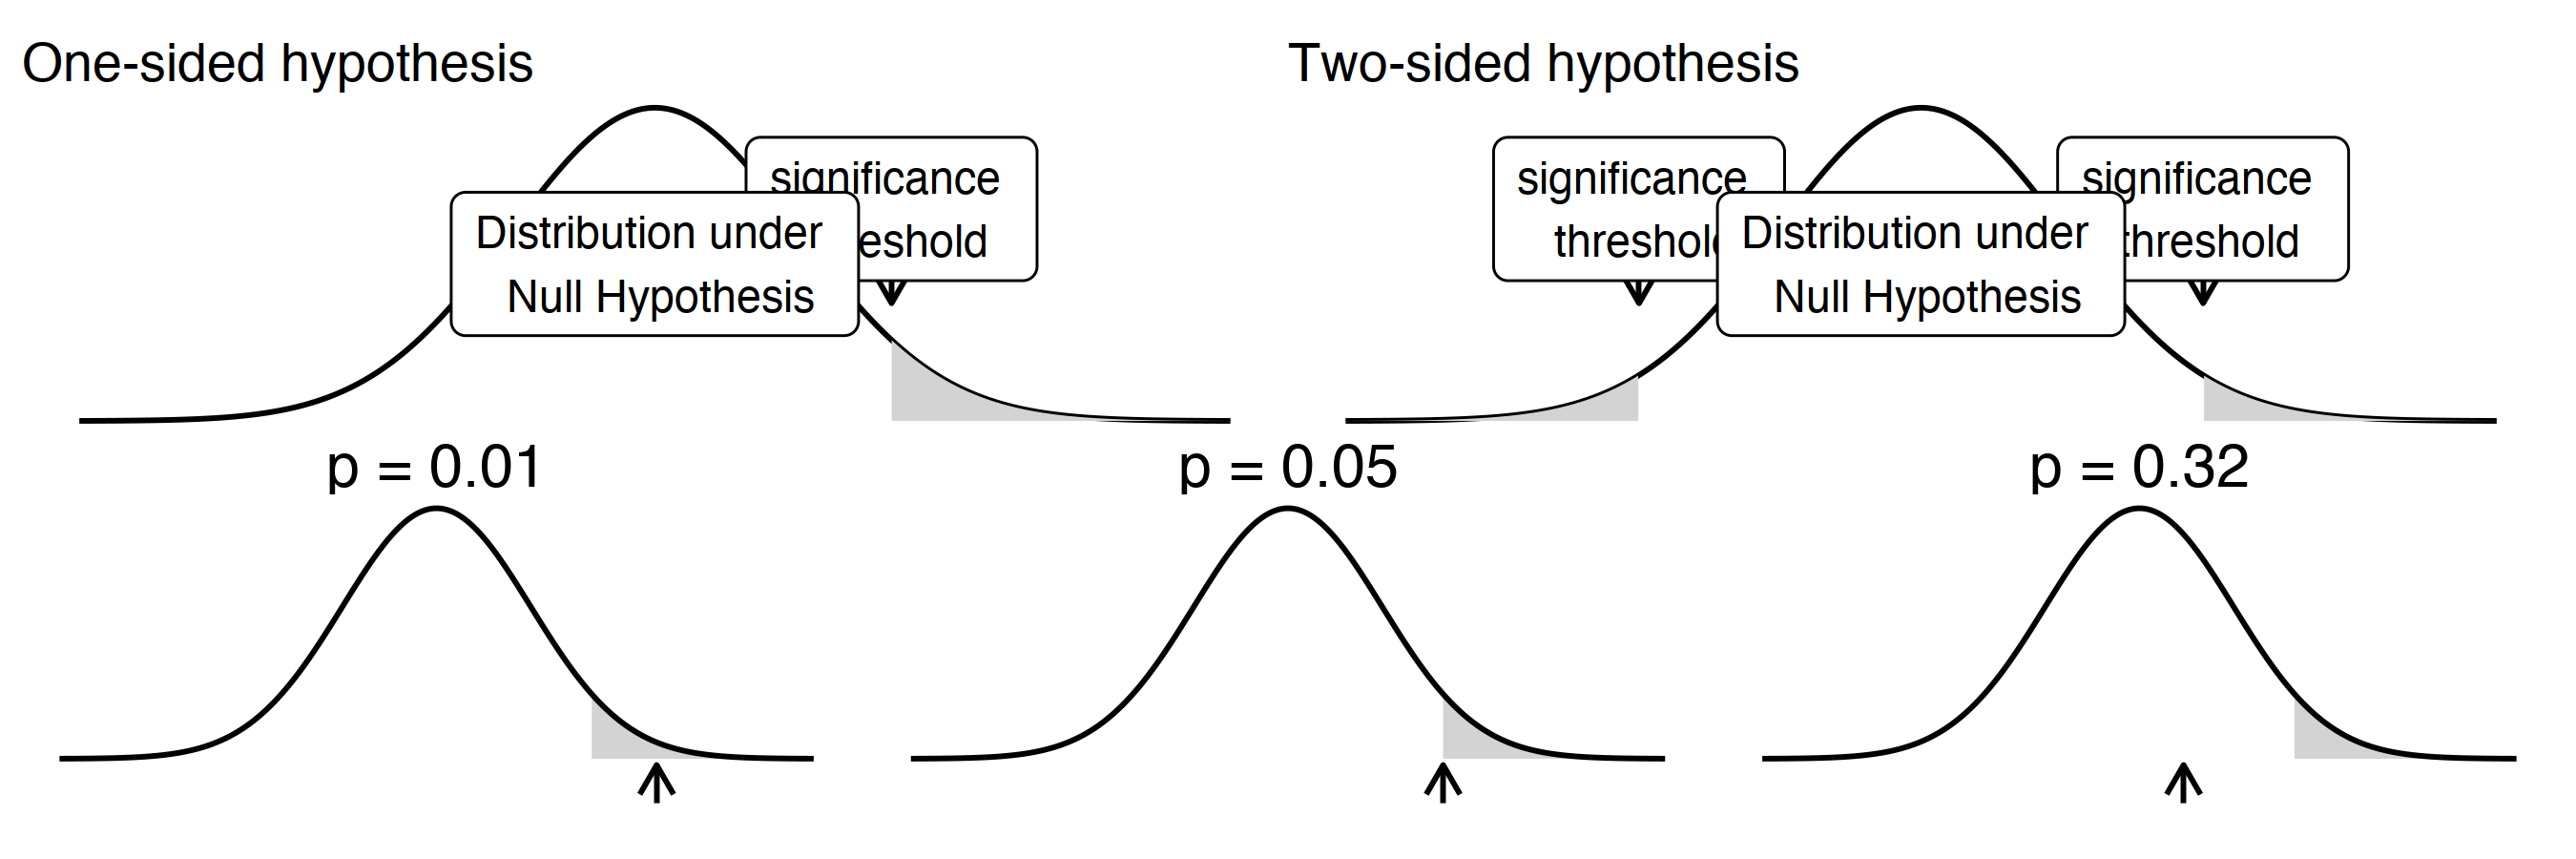
\includegraphics[width=0.8\textwidth]{figures/hypothesis-1} 

}

\caption{Frequentists make binary decisions based on hypothesis tests. Assuming the null distribution, the null hypothesis is rejected if the observed estimand is extreme.}\label{fig:hypothesis}
\end{figure}

Null hypothesis testing is very weird.
It's like answering the question around two corners.
Let's say a researcher wants to prove that a drug prevents migraines.
They test the drug because they expect it to work, so the hypothesis they assume to be true is that patients that take the drug have fewer migraines.
But the null hypothesis is formulated the other way around:
The null hypothesis assumes that the drug has no effect.
Suddenly the goal of the researcher becomes to show that the null hypothesis is false, rather than showing that their hypothesis is correct.
The problem with statistical models is: We can't prove that they are true because our assumptions are not testable.
With frequentist inference, however, we can tell how likely a model result is under a given hypothesis and given the data.
That's why hypothesis tests work by rejection.

P-values allow simple decisions: Is the parameter different from zero?
If yes, frequentists speak of significant effects.
Unfortunately, the entire modeling process is often ultimately reduced to the question of statistical significance.
Achieving a significant result becomes the ultimate goal of a researcher's analysis.
Chasing those small p-values.

\hypertarget{confidence-intervals}{%
\section{Confidence Intervals}\label{confidence-intervals}}

Frequentists use confidence intervals as an alternative to statistical tests.
Hypothesis tests and confidence intervals ultimately lead to the same decisions, but confidence intervals are more informative.
Many statisticians prefer confidence intervals over mere p-values.

Remember that estimators, such as model parameters, are random variables?
That means that estimators have probability distributions.
A confidence interval describes where the mass of that distribution lies.
What percentage of the distribution we want in the confidence interval is again decided by the modeler using an \(\alpha\)-level.
If \(\alpha = 0.05\), then we get a 95\%-confidence interval.
The construction of the confidence interval depends on the probability distribution we have derived for the quantity of interest (coefficient, mean estimate, \ldots).

How are the confidence intervals to be interpreted?
Well, in a frequentist manner, of course!
The ``true'' parameter value is fixed, so it's not a random variable.
To say that the true parameter is in the confidence interval with a 95\% probability would be false.
The true parameter is either in the interval or it's not, we just don't know.
The confidence itself is a random variable since it's derived from data and therefore from other random variables.
So the interpretation of a 95\% confidence interval is:
If we were to repeat the analysis many times, the confidence interval would cover the true value of the quantity of interest 95\% of the time.
Only given that the model assumptions are correct.
As you can see, this is a very frequentist point of view: the confidence interval is interpreted in the context of repeated experiments.

Confidence intervals look different from tests at first glance.
But they are equivalent to the tests:
At least you get the same accept/reject result for the same significance level \(\alpha\).
But the confidence interval contains more information than a simple hypothesis test.
The interval gives the estimate, and lower and upper bounds.
This gives the modeler a better sense of the estimate and its uncertainty.
Rejection of the null hypothesis is equivalent to the null hypothesis being outside of the confidence interval.

\begin{figure}

{\centering 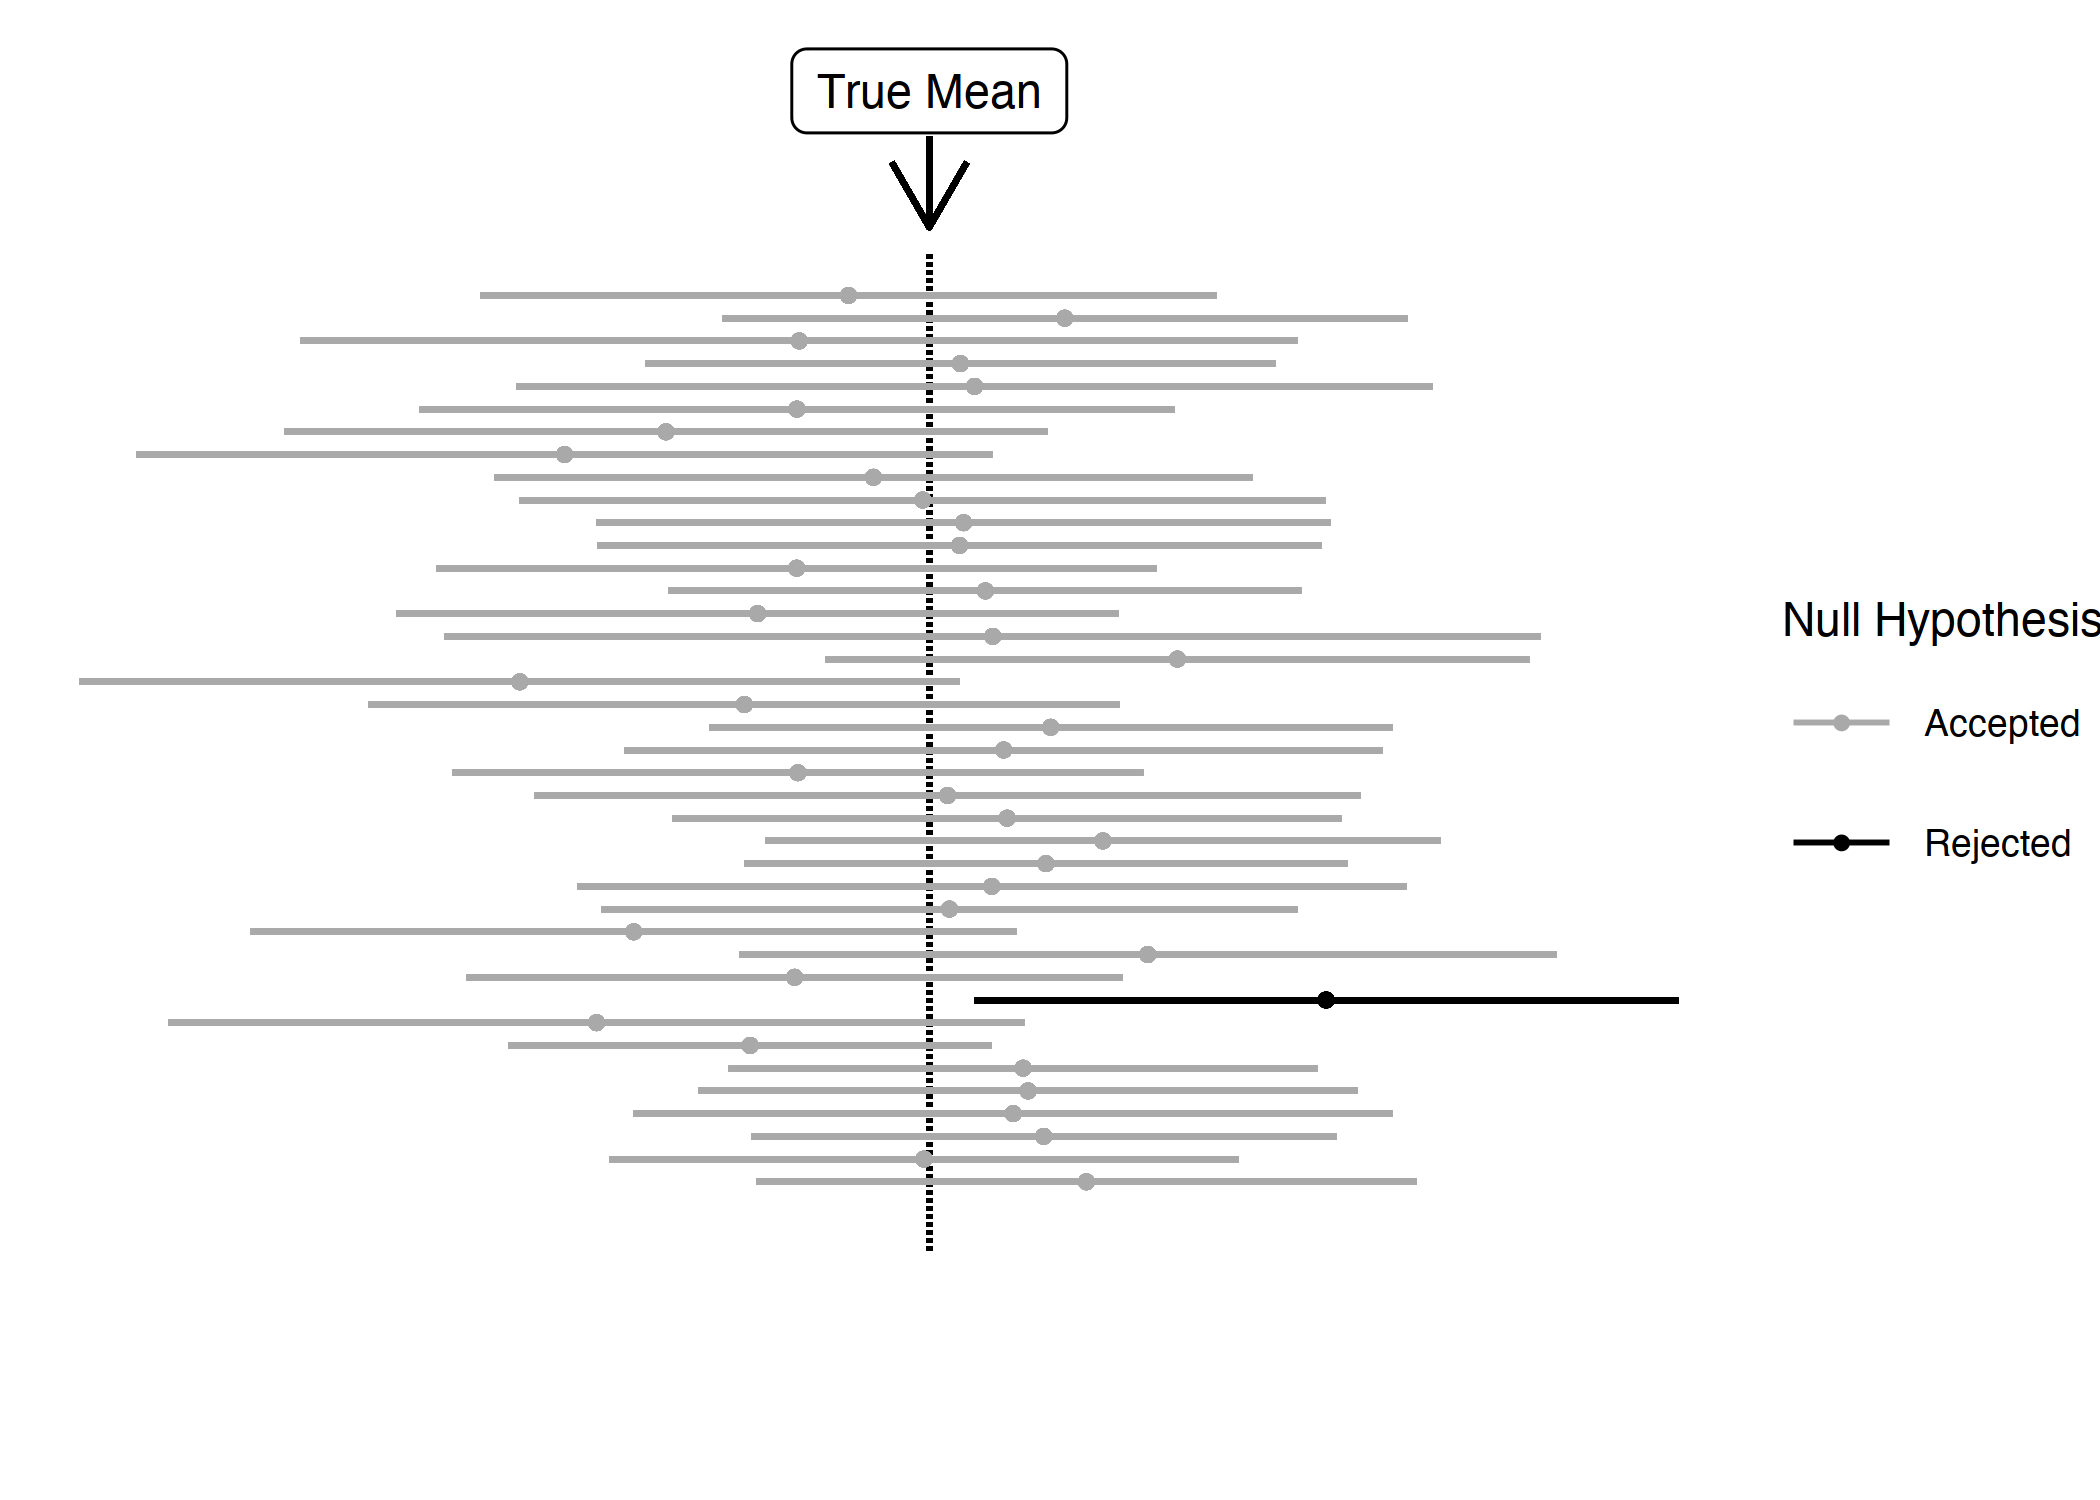
\includegraphics[width=0.8\textwidth]{figures/ci-1} 

}

\caption{100 95\% confidence intervals and the true value.}\label{fig:ci}
\end{figure}

-\textgreater{}

\hypertarget{strengths-1}{%
\section{Strengths}\label{strengths-1}}

\begin{itemize}
\tightlist
\item
  Once you understand frequentist inference, you have the key to understanding most modern research findings. I studied statistics and can now quickly grasp many research papers. For example, to figure out whether I should have knee surgery for my torn meniscus, I read papers comparing knee surgery and physiotherapy alone. All of those papers used frequentist methods, and although I didn't understand everything, I was able to quickly get an idea of their analyses and results.
\item
  Frequentist methods are generally faster to compute than \protect\hyperlink{bayesian}{Bayesian inference} or \protect\hyperlink{supervised-ml}{machine learning}.
\item
  Compared to \protect\hyperlink{bayesian}{Bayesianism}, no prior information about the parameters is required. This makes frequentism more objective.
\item
  Frequentism allows binary decisions (accept/reject hypothesis). This simplicity one of the reasons why it's so popular for scientists and why managers love it.
\item
  Frequentism has all the advantages of the \protect\hyperlink{statistical-modeling}{statistical models} in general: a solid theoretical foundation and an appreciation of the data-generating process.
\item
  When the underlying process is a long-run, repeated experiment, frequentist inference shines. Casino games, model benchmarks, \ldots{}
\end{itemize}

\hypertarget{limitations-1}{%
\section{Limitations}\label{limitations-1}}

\begin{itemize}
\tightlist
\item
  Frequentism invites \textbf{over-simplification of answers}into simple yes/no-answers. Simplification into the question of results ``significantly'' deviate from the null hypothesis. Reducing models to binary decisions obscures critical model assumptions and the difficult trade-offs that had to be made for the analysis.
\item
  Focusing on p-values encourages \textbf{p-hacking}: the either conscious or unconscious search for ``positive'' results. Guided by the lure of a significant result, researchers and data scientists may play around with their analysis until the p-value in question is small enough. With \(\alpha\)-level of 0.05, 1 in 20 null hypotheses are falsely rejected. P-hacking increases this percentage of false positive findings.
\item
  Similarly, if the analysis is exploratory rather than hypothesis-driven, a naive frequentist approach may produce many false positive findings. Look again at figure \ref{fig:ci}: Imagine these were confidence intervals for different variables. Again, for \(\alpha = 0.05\), we would expect 1 in 20 hypothesis tests to yield false positives. Now imagine a data scientist testing hundreds of hypothesis tests. This problem is called the multiple testing problem. There are solutions, but they are not always used and multiple testing can be very subtle.
\item
  The frequentist interpretation of probability is very awkward when it comes to confidence intervals and p-values. They are commonly misinterpreted. Arguably, frequentist confidence intervals are not what practitioners want. \protect\hyperlink{bayesian}{Bayesian} credibility intervals are more aligned with the natural interpretation of uncertainty.
\item
  Frequentist analysis depends not only on the data, but also on the experimental design. This is a violation of the likelihood principle that says that all information about the data must be contained in the likelihood, see example in \protect\hyperlink{likelihoodism}{chapter on likelihoodism}.
\item
  Frequentist probability can fail in the simplest scenarios: Imagine you are modeling the probability of rain in August. The data only has 20 August days, all of which are without rain. The frequentist answer is that there is absolutely no chance that it will ever rain in August. The frequentist recommendation is that to collect more data if we want a better answer. \protect\hyperlink{bayesian}{Bayesianism} offers a solution to involve prior information for such estimates.
\item
  There is an ``off-the-shelf''-mentality among users of frequentist inference. Instead of carefully adapting a probability model to the data, an off-the-shelf statistical test or statistical model is chosen. The choice is based on just a few properties of the data. For example, there are popular flow charts of choosing an appropriate statistical test.
\item
  Frequentist statistics says nothing about causality except that ``correlation does not imply causation''.
\end{itemize}

\hypertarget{bayesian}{%
\chapter{Bayesian Inference}\label{bayesian}}

\begin{itemize}
\tightlist
\item
  Interprets probability as degree of belief and learning from data as updating that belief.
\item
  Model parameters are random variables with a prior distribution. Goal: posterior distribution.
\item
  A \protect\hyperlink{statistical-modeling}{statistical modeling mindset} with \protect\hyperlink{frequentism}{frequentism} and \protect\hyperlink{likelihoodism}{likelihoodism} as alternatives.
\end{itemize}

\textbf{This chapter is under construction! Stay tuned.}

\hypertarget{likelihoodism}{%
\chapter{Likelihoodism}\label{likelihoodism}}

\begin{itemize}
\tightlist
\item
  Focused on the likelihood, follows the likelihood principle.
\item
  Does not assume that parameters are random variables.\\
\item
  A \protect\hyperlink{statistical-modeling}{statistical modeling mindset} with \protect\hyperlink{frequentism}{frequentism} and \protect\hyperlink{bayesianism}{Bayesianism} as alternatives.
\end{itemize}

\textbf{This chapter is under construction! Stay tuned.}

\hypertarget{causal}{%
\chapter{Causal inference}\label{causal}}

\begin{itemize}
\tightlist
\item
  Assumes that random variables are connected through cause and effect.
\item
  Builds a causal model from which statistical estimators are derived.
\item
  A \protect\hyperlink{statistical-modeling}{statistical modeling mindset} that adds causality to \protect\hyperlink{frequentism}{frequentist} and \protect\hyperlink{bayesian}{Bayesian} inference.
\end{itemize}

\textbf{This chapter is under construction! Stay tuned.}

\hypertarget{supervised-ml}{%
\chapter{Supervised Machine Learning}\label{supervised-ml}}

\begin{itemize}
\tightlist
\item
  Focus on prediction rather than understanding the data-generating process.
\item
  Focus on loss minimization and evaluation with unseen data.
\item
  Alternative to the random variable focused \protect\hyperlink{statistical-modeling}{statistical modeling mindset}, but also draws heavily from it, method-wise.
\end{itemize}

\textbf{This chapter is under construction! Stay tuned.}

\hypertarget{deep-learning}{%
\chapter{Deep Learning}\label{deep-learning}}

\begin{itemize}
\tightlist
\item
  Neural networks based on stacking various layers of neurons.
\item
  World of feature embeddings, transfer learning and foundation models.
\item
  A machine learning mindset, can also be used for \protect\hyperlink{supervised-ml}{supervised learning}.
\end{itemize}

\textbf{This chapter is under construction! Stay tuned.}

\hypertarget{references}{%
\chapter*{References}\label{references}}


Blei, David M., Alp Kucukelbir, and Jon D. McAuliffe. ``Variational inference: A review for statisticians.'' Journal of the American statistical Association 112, no. 518 (2017): 859-877.

For continuous variables like water intake, technically we may not interpret probability density functions at a certain value, like P(intake = 2.5 liter) as probability. Instead we have to take the integral, for example over the range of 2.4 to 2.6 liters and then may interpret as the probability.

Gandenberger, Greg. Why I am not a likelihoodist. Ann Arbor, MI: Michigan Publishing, University of Michigan Library, 2016.

Hernán, Miguel A., and James M. Robins. ``Causal inference.'' (2010): 2.

ISyE8843A, Brani Vidakovic Handout. ``1 The Likelihood Principle.''

Ioannidis, John PA. ``Why most published research findings are false.'' PLoS medicine 2, no. 8 (2005): e124.

Judea, Pearl. ``An introduction to causal inference.'' The International Journal of Biostatistics 6, no. 2 (2010): 1-62..

Kao, WH Linda, Ian B. Puddey, Lori L. Boland, Robert L. Watson, and Frederick L. Brancati. ``Alcohol consumption and the risk of type 2 diabetes mellitus: atherosclerosis risk in communities study.'' American journal of epidemiology 154, no. 8 (2001): 748-757.

Pearl, Judea. ``The do-calculus revisited.'' arXiv preprint arXiv:1210.4852 (2012).

Savage, Leonard J. The foundations of statistics. Courier Corporation, 1972.

Some approaches don't assume a closed form distribution. For example the Cox proportional hazards model. For the Cox model, we optimize the partial likelihood. These approaches are called semiparametric.

Weisberg, Michael. Simulation and similarity: Using models to understand the world. Oxford University Press, 2012.

Wynants, Laure, Ben Van Calster, Gary S. Collins, Richard D. Riley, Georg Heinze, Ewoud Schuit, Marc MJ Bonten et al.~``Prediction models for diagnosis and prognosis of covid-19: systematic review and critical appraisal.'' bmj 369 (2020).

Yang, Ruoyong, and James O. Berger. A catalog of noninformative priors. Durham, NC, USA: Institute of Statistics and Decision Sciences, Duke University, 1996.

\printindex
\thispagestyle{empty}


\end{document}
